%\documentclass[letterpaper, 12pt, parskip=full,DIV=10]{scrartcl}
% The next three lines are temporary, for todo notes, remove after notes are removed
\documentclass[letterpaper, 12pt, parskip=full,]{scrartcl}
\setlength{\marginparwidth}{4.5cm}
\usepackage[top=2.5cm, bottom=2.5cm, left=1.5cm, right=5cm]{geometry}
% Title and Subtitle added in .tex file

\title{Optimal Policies to Battle the Coronavirus ``Infodemic'' Among Social Media Users in Sub-Saharan Africa}
\subtitle{Preanalysis plan}
\author{Molly Offer-Westort, Leah R. Rosenzweig, Susan Athey}
\date{\today}

% USE: %\documentclass[letterpaper, 12pt, parskip=full,]{scrartcl}

\RequirePackage{etex}

% Graphics
\RequirePackage{graphicx}
\RequirePackage{epsfig}
\RequirePackage{psfrag}
\RequirePackage{wrapfig}
\RequirePackage[all]{xy}
\RequirePackage{listings}
\RequirePackage{verbatim} 
\RequirePackage{color} 
% Bold the 'Figure #' in the caption and separate it from the title/caption with a period
% Captions will be left justified
\RequirePackage[aboveskip=1pt,labelfont=bf,labelsep=period,justification=raggedright,singlelinecheck=off]{caption}


% Tables
\RequirePackage{float}
\RequirePackage{rotating}
\RequirePackage{array}
%\RequirePackage{minipage}
\RequirePackage{booktabs,threeparttable}

% Author
\RequirePackage[blocks]{authblk}
\renewcommand\Affilfont{\small}
\setlength{\affilsep}{0em}

\lstset{breaklines=true,basicstyle=\footnotesize\ttfamily}

% Document formatting
%\RequirePackage{fullpage}
\RequirePackage{setspace}
\RequirePackage{mathptmx}
\RequirePackage[hyphens]{url}
\RequirePackage{microtype} 
\RequirePackage[utf8x]{inputenc}
\RequirePackage{enumitem}
\setlist[itemize]{noitemsep, topsep=0pt}
\RequirePackage[colorinlistoftodos, textsize=footnotesize, color=blue!20!white]{todonotes} % adding to-do notes in working file
%\addtokomafont{disposition}{\normalfont\bfseries} % article fonts
%\setkomafont{descriptionlabel}{\normalfont\bfseries} % article fonts

% Bibliography and citation formatting
\RequirePackage[colorlinks=true, citecolor=blue]{hyperref}

\RequirePackage{nameref}
\RequirePackage[round]{natbib} 
\bibliographystyle{chicago}

% Title and Subtitle added in .tex file
%\author{Molly Offer-Westort}
%\date{\today}

\makeatletter %Set \Title reference
\let\Title\@title
\makeatother

\makeatletter %Set \Subtitle reference
\let\Subtitle\@subtitle
\makeatother

\makeatletter %Set \Author reference
\let\Author\@author
\makeatother

% Header and Footer
\RequirePackage{scrlayer-scrpage}
%\ihead{\textbf{\Title} }
%\ohead{\Author}

\RequirePackage{lastpage}
%\cfoot[]{}
%\ofoot[]{\thepage\ of \pageref{LastPage}}
\pagestyle{scrheadings}
%\setkomafont{pageheadfoot}{\small}
\RequirePackage{footnote}
\deffootnote[1.5em]{.5em}{1em}{\textsuperscript{\thefootnotemark}}


% Equation formatting
\RequirePackage{amsmath,amssymb,amsfonts} 
\RequirePackage{amsthm}
\RequirePackage{bbm}
\RequirePackage{array}
\newcommand\numberthis{\addtocounter{equation}{1}\tag{\theequation}}

\newtheorem{theorem}{Theorem}[section]
\newtheorem{lemma}{Lemma}[section]
\newtheorem{prop}{Proposition}[section]
\newtheorem{corollary}{Corollary}[section]
\newtheorem{hypothesis}{Hypothesis}


% Shortcuts
\newcommand{\nn}{\nonumber}

% Define new characters
\def\Var{{\textrm{Var}}\,}
\def\V{{\textrm V}\,}
\def\E{{\textrm E}\,}
\def\arg{{\textrm {arg} }\,}
\def\Cov{{\textrm{Cov} }\,}
\def\Cor{{\textrm{Cor} }\,}
\def\N{{\textrm N}\,}
\def\Supp{{\textrm {Supp} }\,}
\DeclareMathOperator*{\argmin}{arg\,min}
\DeclareMathOperator*{\argmax}{arg\,max}

%--------------------------------------------------------------------------
% Math boldface shortcuts, etc. ----------------------------------
%--------------------------------------------------------------------------
\newcommand{\A}{\mathbf{A}}\newcommand{\B}{\mathbf{B}}\newcommand{\C}{\mathbf{C}}
\newcommand{\D}{\mathbf{D}}\newcommand{\F}{\mathbf{F}}\newcommand{\G}{\mathbf{G}}
\newcommand{\HB}{\mathbf{H}}\newcommand{\I}{\mathbf{I}}\newcommand{\J}{\mathbf{J}}
\newcommand{\K}{\mathbf{K}}\newcommand{\Lb}{\mathbf{L}}\newcommand{\M}{\mathbf{M}}
\newcommand{\NB}{\mathbf{N}}\newcommand{\OB}{\mathbf{O}}\newcommand{\PB}{\mathbf{P}}
\newcommand{\Q}{\mathbf{Q}}\newcommand{\R}{\mathbf{R}}\newcommand{\SB}{\mathbf{S}}
\newcommand{\T}{\mathbf{T}}\newcommand{\U}{\mathbf{U}}%\newcommand{\V}{\mathbf{V}}
\newcommand{\W}{\mathbf{W}}\newcommand{\X}{\mathbf{X}}\newcommand{\Y}{\mathbf{Y}}
\newcommand{\Z}{\mathbf{Z}}

\newcommand{\aB}{\mathbf{a}}\newcommand{\bB}{\mathbf{b}}\newcommand{\cB}{\mathbf{c}}
\newcommand{\dB}{\mathbf{d}}\newcommand{\e}{\mathbf{e}}\newcommand{\f}{\mathbf{f}}
\newcommand{\g}{\mathbf{g}}\newcommand{\h}{\mathbf{h}}\newcommand{\iB}{\mathbf{i}}
\newcommand{\jB}{\mathbf{j}}\newcommand{\kB}{\mathbf{k}}\newcommand{\lB}{\mathbf{l}}
\newcommand{\m}{\mathbf{m}}\newcommand{\n}{\mathbf{n}}\newcommand{\oB}{\mathbf{o}}
\newcommand{\p}{\mathbf{p}}\newcommand{\q}{\mathbf{q}}\newcommand{\rB}{\mathbf{r}}
\newcommand{\s}{\mathbf{s}}\newcommand{\tB}{\mathbf{t}}\newcommand{\uB}{\mathbf{u}}
\newcommand{\vB}{\mathbf{v}}\newcommand{\w}{\mathbf{w}}\newcommand{\x}{\mathbf{x}}
\newcommand{\y}{\mathbf{y}}\newcommand{\z}{\mathbf{z}}

\def\AA{{\mathbb A}}\def\BB{{\mathbb B}}\def\CC{{\mathbb C}}
\def\DD{{\mathbb D}}\def\EE{{\mathbb E}}\def\FF{{\mathbb F}}
\def\GG{{\mathbb G}}\def\HH{{\mathbb H}}\def\II{{\mathbb I}}
\def\JJ{{\mathbb J}}\def\KK{{\mathbb K}}\def\LL{{\mathbb L}}
\def\MM{{\mathbb M}}\def\NN{{\mathbb N}}\def\OO{{\mathbb O}}
\def\PP{{\mathbb P}}\def\QQ{{\mathbb Q}}\def\RR{{\mathbb R}}
\def\SS{{\mathbb S}}\def\TT{{\mathbb T}}\def\UU{{\mathbb U}}
\def\VV{{\mathbb V}}\def\WW{{\mathbb W}}\def\XX{{\mathbb X}}
\def\YY{{\mathbb Y}}\def\ZZ{{\mathbb Z}}

\RequirePackage{euscript}
\let\muchmore= \gg
\let\muchless= \ll
\let\typewriter=\tt  % for turning on the typewriter font
\def\aa{{\EuScript A}}\def\bb{{\EuScript B}}\def\cc{{\EuScript C}}\def\dd{{\EuScript D}}
\def\ee{{\EuScript E}}\def\ff{{\EuScript F}}\def\gg{{\EuScript G}}\def\hh{{\EuScript H}}
\def\ii{{\EuScript I}}\def\jj{{\EuScript J}}\def\kk{{\EuScript K}}\def\ll{{\EuScript L}}
\def\mm{{\EuScript M}}\def\nn{{\EuScript N}}\def\oo{{\EuScript O}}\def\pp{{\EuScript P}}
\def\qq{{\EuScript Q}}\def\rr{{\EuScript R}}\def\ss{{\EuScript S}}\def\tt{{\EuScript T}}
\def\uu{{\EuScript U}}\def\vv{{\EuScript V}}\def\ww{{\EuScript W}}\def\xx{{\EuScript X}}
\def\yy{{\EuScript Y}}\def\zz{{\EuScript Z}}

\newcommand{\Beta}{\boldsymbol{\beta}}
\newcommand{\btheta}{\boldsymbol{\theta}}
\newcommand{\bgamma}{\boldsymbol{\gamma}}
\newcommand{\bpi}{\boldsymbol{\pi}}
\newcommand{\arrowp}{\stackrel{p}{\rightarrow}}
\newcommand{\0}{\mathbf{0}}
\newcommand{\bP}{\mathbf{P}}

\newcommand\independent{\protect\mathpalette{\protect\independenT}{\perp}}
\def\independenT#1#2{\mathrel{\rlap{$#1#2$}\mkern2mu{#1#2}}}


\newcommand{\indep}{\perp\!\!\!\!\perp}

\thispagestyle{plain}



\begin{document}%
\normalsize%
\maketitle%
\tableofcontents%
\clearpage%


\centerline{\textbf{ABSTRACT}}
\begin{abstract}
Alongside the outbreak of the new coronavirus, much of the world’s population is also experiencing an “infodemic” -- the spread of myths and hoax cures related to the virus through online media outlets and social media platforms. While many false cures are largely harmless (e.g., drinking lemon water), others have potentially devastating consequences, such as misuse of chloroquine. As a result, governments struggling to prepare healthcare systems and encourage citizens to comply with best practices also need to tackle misinformation. Building upon the experimental literature on combating fake news, we evaluate the effect of interventions designed to decrease sharing of false COVID-19 cures. Using Facebook advertisements to recruit social media users in Kenya and Nigeria, we deliver our interventions using a Facebook Messenger chatbot, allowing us to observe treatment effects in a realistic setting. Using a contextual adaptive experimental design to sequentially assign treatment probabilities, we are able to learn the optimal contextual policy, and minimize assignment to ineffective or counter-productive interventions within the experiment. Analyzing heterogeneity in treatment effects allows us to learn whether different interventions are more effective for different people, improving our understanding of how to tackle harmful misinformation during an ongoing health crisis. Finally, we bring comparative data to a global problem for which the existing research has largely been limited to the U.S. and Europe. This pre-analysis plan describes the research design and outlines the key hypotheses that we will evaluate.
\end{abstract}





\section{Motivation and Research Questions}

% infodemic - what it is
Alongside the outbreak of the novel coronavirus (SARS-CoV-2), much of the world's population is also experiencing an ``infodemic'' -- the spread of misinformation related to the virus. The COVID-19 misinformation spreading on social media platforms involve a range of topics including rumors about the origin of the virus, government activities, scam opportunities for aid, and hoax cures. In some places, citizens remain in disbelief and denial of the very existence of the virus.\footnote{\url{https://www.bbc.com/news/world-africa-53403818}} 

%  covid misinfo spreading! / shared
Much like the actual virus, COVID-19 misinformation is not bounded by state borders. Though the infection rate ($R_0$) of these falsities is difficult to calculate, if the spread follows the trajectory of other types of online information, we should expect COVID-19 misinformation to spread faster and farther than true information \citep{vosoughi2018spread}. For instance, misinformation about the Zika virus was three times more likely to be shared on social media than verified information on several social media sites \citep{sharma2017zika}. Indeed, recent research on COVID-19 conspiracy theories suggests that these stories had a higher virality than neutral or debunking stories \citep{HKS_whatsapp}. %
 

% infodemic - why it matters --> real consequences
We might be particularly worries about the spread of COVID-19 hoax cures because they can be deadly. Purported cures for COVID-19 that have circulated on social media include both benign recommendations, such as drinking lemon water and inhaling steam, as well as those that can have devastating consequences if adopted, such as misusing chloroquine or drinking bleach. In Iran, dozens of people died from alcohol poisoning after ingesting methanol supposedly due to the rumor that alcohol could prevent coronavirus.\footnote{\href{https://nationalpost.com/news/world/rumours-that-alcohol-kills-covid-19-leaves-21-iranians-dead-from-poisoning}{Bloomberg News}, Mar. 10, 2020.} In Nigeria, multiple people were hospitalized for chloroquine poisoning following statements by president Trump suggesting the medication could be used to treat COVID-19.\footnote{\href{https://www.cnn.com/2020/03/23/africa/chloroquine-trump-nigeria-intl/index.html}{CNN}, Mar. 23, 2020.} 

Though identifying the causal link between online rumors and offline behaviors is challenging, online information has been shown to have offline consequences. For instance, activity on social media and the internet more generally has been linked to offline behaviors such as hate crimes \citep{muller2019fanning, chan2016internet}. Health misinformation can have particularly harmful consequences for one's wellbeing and risk of mortality \citep{swire2020public}. As a result of the ``infodemic'', governments struggling to prepare health care systems and encourage citizens to comply with best practices are also struggling to tackle a pandemic of online misinformation.


% why it's hard to combat:
% what's new about this context
Curbing the spread of online misinformation is challenging in ``normal'' times, but is particularly difficult in the context of a global pandemic. Unlike political misinformation covid-19 misinformation arises in an uncertain environment where facts are rapidly-changing as more information and evidence become available and where longstanding preexisting beliefs do not exist. %(in contrast to say beliefs about climate change, etc.) 
The human need for certainty, security, and stability is strong \textbf{(CITE)}. Thus, people turn to multiple sources for health information in addition to scientific experts \citep{swire2020public}.  % -- nowadays ppl get health info from many sources --> covid times harder to 
% swire - health: similarly hard to evaluate "cause"/"effect" of misinfo online
Also worrying, one study found that COVID-19 misinformation on whatsapp continued to circulate among users in India and Brazil even \textit{after} the information had been debunked by fact-checking organizations. Given the absence of a vaccine or full proof prevention method, it is unsurprising that people are searching in desperation for any kind of ``cure,'' even those that have been labelled as false, and sharing these with their friends and family. Given the importance of understanding how to curb the spread of these kinds of false information, this project seeks to understand what different types of people are influenced by different mechanisms targeted to reduce the spread of false information.

%Furthermore, during the COVID-19 pandemic, there has been an uptick in rumours and conspiracies spreading through online platforms (Ferrara, 2020). 

\textbf{More context motivation here + Section 3.3...}


% what we do 
This project evaluates the effect of interventions designed to decrease sharing of false COVID-19 cures. Using Facebook advertisements to recruit social media users in Kenya and Nigeria, we deliver our interventions using a Facebook Messenger chatbot, allowing us to observe treatment effects in a realistic setting and environment where such stories have appeared. Other studies have demonstrated that sharing behavior in online surveys mirror those of real-world social media users \citep{mosleh2020self}. We test interventions targeted at both the respondent level, such as tips for spotting fake news, a video training and nudges, as well as headline-level treatments, such as ``false'' tags and related articles. All of the treatments are described in Table~\ref{tab:treatments}. 

Using a contextual adaptive experimental design, we sequentially assign treatment probabilities to privilege assignment to the most effective interventions, and minimize assignment to ineffective or counter-productive interventions. Our aim is to learn an optimal contextual policy that will assign respondents the intervention that is most effective for them, conditional on their covariate profile. Exploring heterogeneity in treatment effects allows us to learn whether different interventions are more effective for different people, improving our understanding of how to tackle harmful misinformation during an ongoing health crisis. 

% how we build on existing lit
This work builds on the experimental literature on combating fake news in several important ways. First, we examine several prominent interventions that have proven successful in other studies and in other settings using an adaptive design to observe the best intervention policy.\todo{bring in heterogeneity focus here.} Second, we bring comparative data to a global problem. Despite the global nature of the ``infodemic,'' much of the existing research has been focused on the Global North, particularly the United States \citep{pennycook2020fighting, bursztyn2020misinformation}.\footnote{Two recent exceptions from sub-Saharan Africa include a field experiment in Zimbabwe using Whatsapp messages from a trusted NGO  to counter COVID misinformation \citep{bowles2020center} and a recent survey among traders in Lagos, Nigeria looking at the correlates of belief in COVID-related misinformation \citep{Grossman2020}.} This pre-analysis plan describes the research design, outlines the key hypotheses that we will evaluate, and details our approach to analysis.




\section{Case Selection and Stimuli}
% Why kenya + Nigeria?

We examine these questions using a study focused on online social media users in two major English-language hubs of online communication in sub-Saharan Africa, Kenya and Nigeria.  Collectively, Facebook estimates there are 30-35 million Facebook users who are 18 years and older from these two countries (as reported on \href{https://www.facebook.com/business/insights/tools/audience-insights?ref=ens_rdr}{Facebook's advertising platform}). Misinformation and fake news are major problems in these countries. AfricaCheck.org, a third party verification site, has offices in both countries and has recently created pages devoted to coronavirus-related misinformation circulating online. From January to March, the number of English-language fact-checks increased by more than 900\% worldwide \citep{brennen2020types}, demonstrating the prevalence of this kind of content and the availability of verified coronavirus-related information.  Figure \ref{fig:poynter} illustrates the volume of fact checks that appear in \url{poynter.org}'s global coronavirus facts database, which demonstrates that Kenya and Nigeria are main factcheck sources on the continent. Thus, there is a large database of verified information from which we can draw stimuli for our experiment in these two countries. 

\begin{figure}[!htb]
\centering
\caption{Map illustrating the volume of fact-checks in \url{poynter.org}'s global coronavirus facts database.}
\label{fig:poynter}
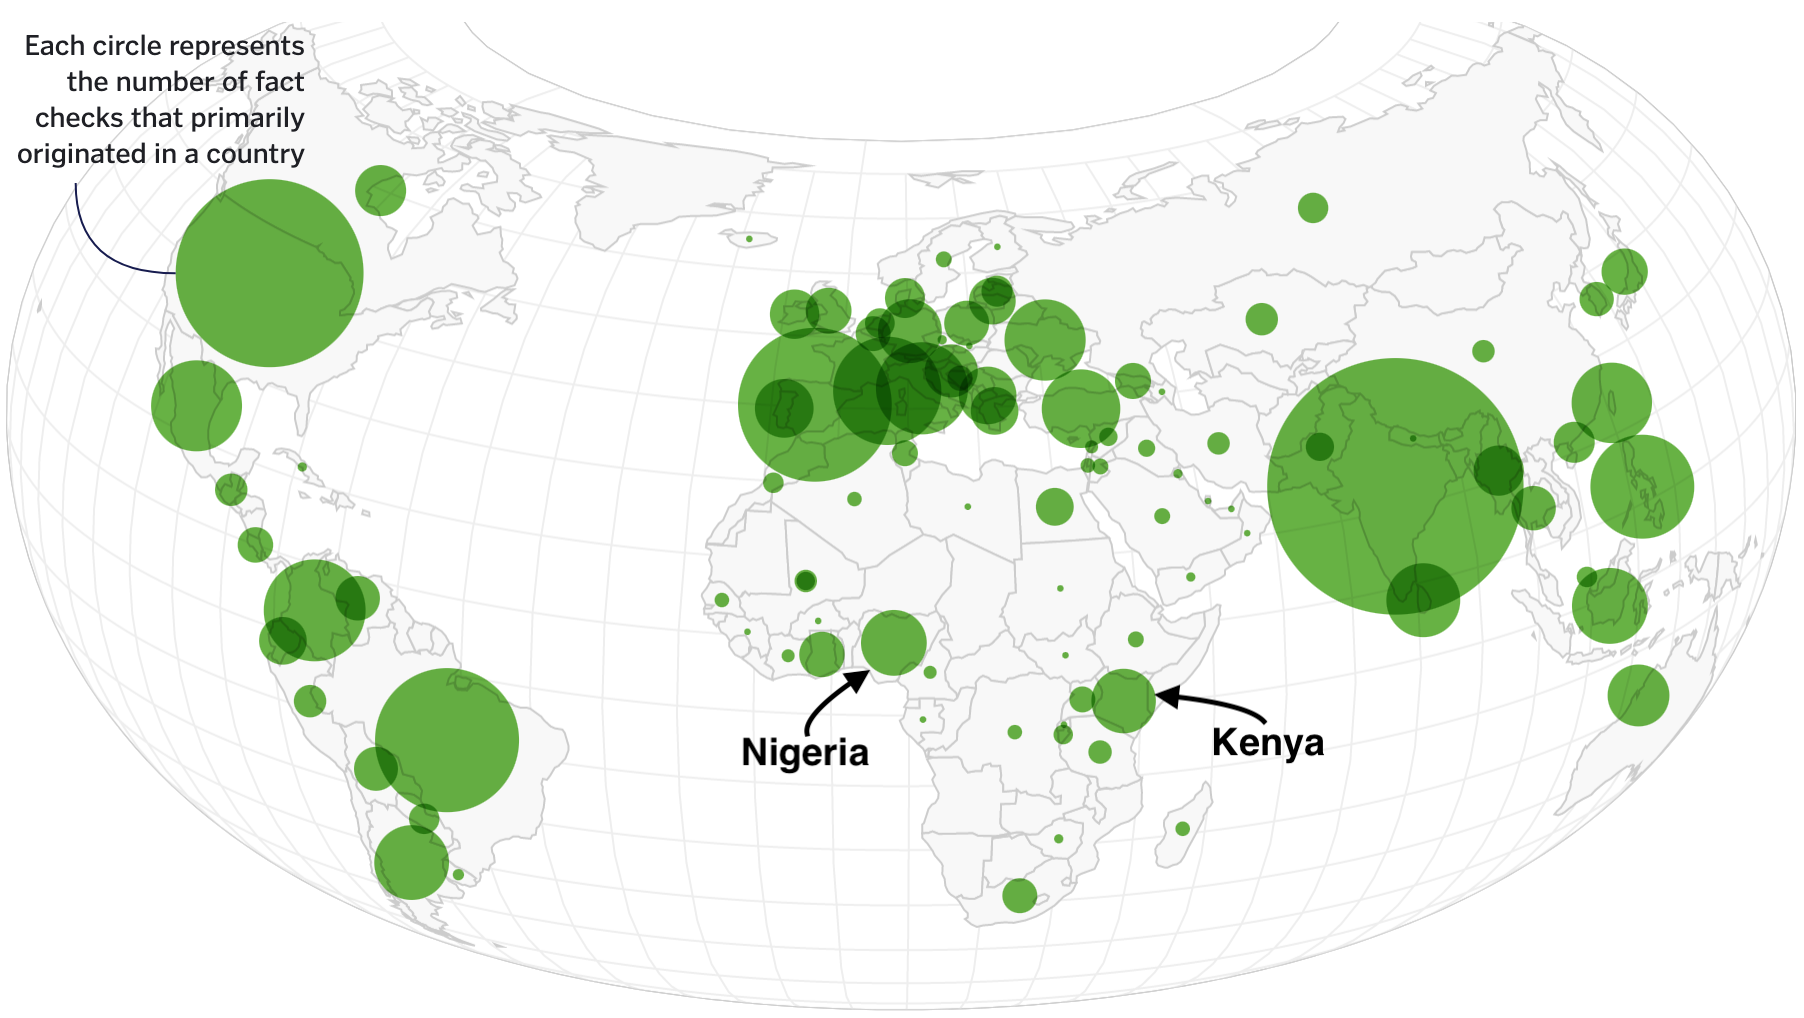
\includegraphics[width=.95\textwidth]{poynter2.png}
\end{figure}

For this experiment, we focus on COVID-19 prevention and cure-related information because this comprises a large proportion of the overall coronavirus-related information that has been fact-checked by experts (see Figure \ref{fig:poynter_cures}) and also serves as some of the most dangerous misinformation. Some hoax cures, when adopted, can be deadly. Moreover, even if not adopted when claims about the existence of a cure circulate widely they may deter people from taking preventative measures. We acknowledge that interventions will likely need to be specific to the particular type of misinformation being targeted, whether political, health-related, etc. The focus of this paper is on prevention and cure-related (mis)information that is immediately relevant for the ongoing pandemic. 
%\todo{Should this be moved to a new 3.3.2 Stimuli section?} - kept here and changed section heading

To collect stimuli we adopted several criteria to search for both false and true pieces of information related to coronavirus prevention techniques and COVID-19 cures. First, we searched AFP, Poynter, and AfricaCheck website for any of this type of misinformation that had been checked by these organizations that appeared online in Kenya and Nigeria since the start of the pandemic in early March 2020. Second, we collected WHO myth-buster infographics that directly countered the misinformation items we found. We also collected prevention messaging from the Nigeria Center for Disease Control, National Emergency Response Committee in Kenya, and the Ministry of Health in both countries, as these are the main government entities combating the spread of the disease in these countries and official sources of information. Our full set of stimuli for each country is provided in Appendix~\ref{appendis:stimuli}.\footnote{In addition to realism of the study, we use actual stimuli circulating online to avoid manufacturing our own ``cures'' and adding to the spread of online misinformation. Given that we use real media posts, some of our respondents may be familiar with these stories. To examine whether people were differentially discerning \citep{nyhan2020facts} or had different sharing preferences because they had previously seen these stimuli, at the end of the survey, before the debrief, we ask respondents whether they had previously seen the stimuli.}





\begin{figure}[t]
\centering
\caption{Map illustrating the volume of COVID-19 cure-related fact-checks in \url{poynter.org}'s global coronavirus database.}
\label{fig:poynter_cures}
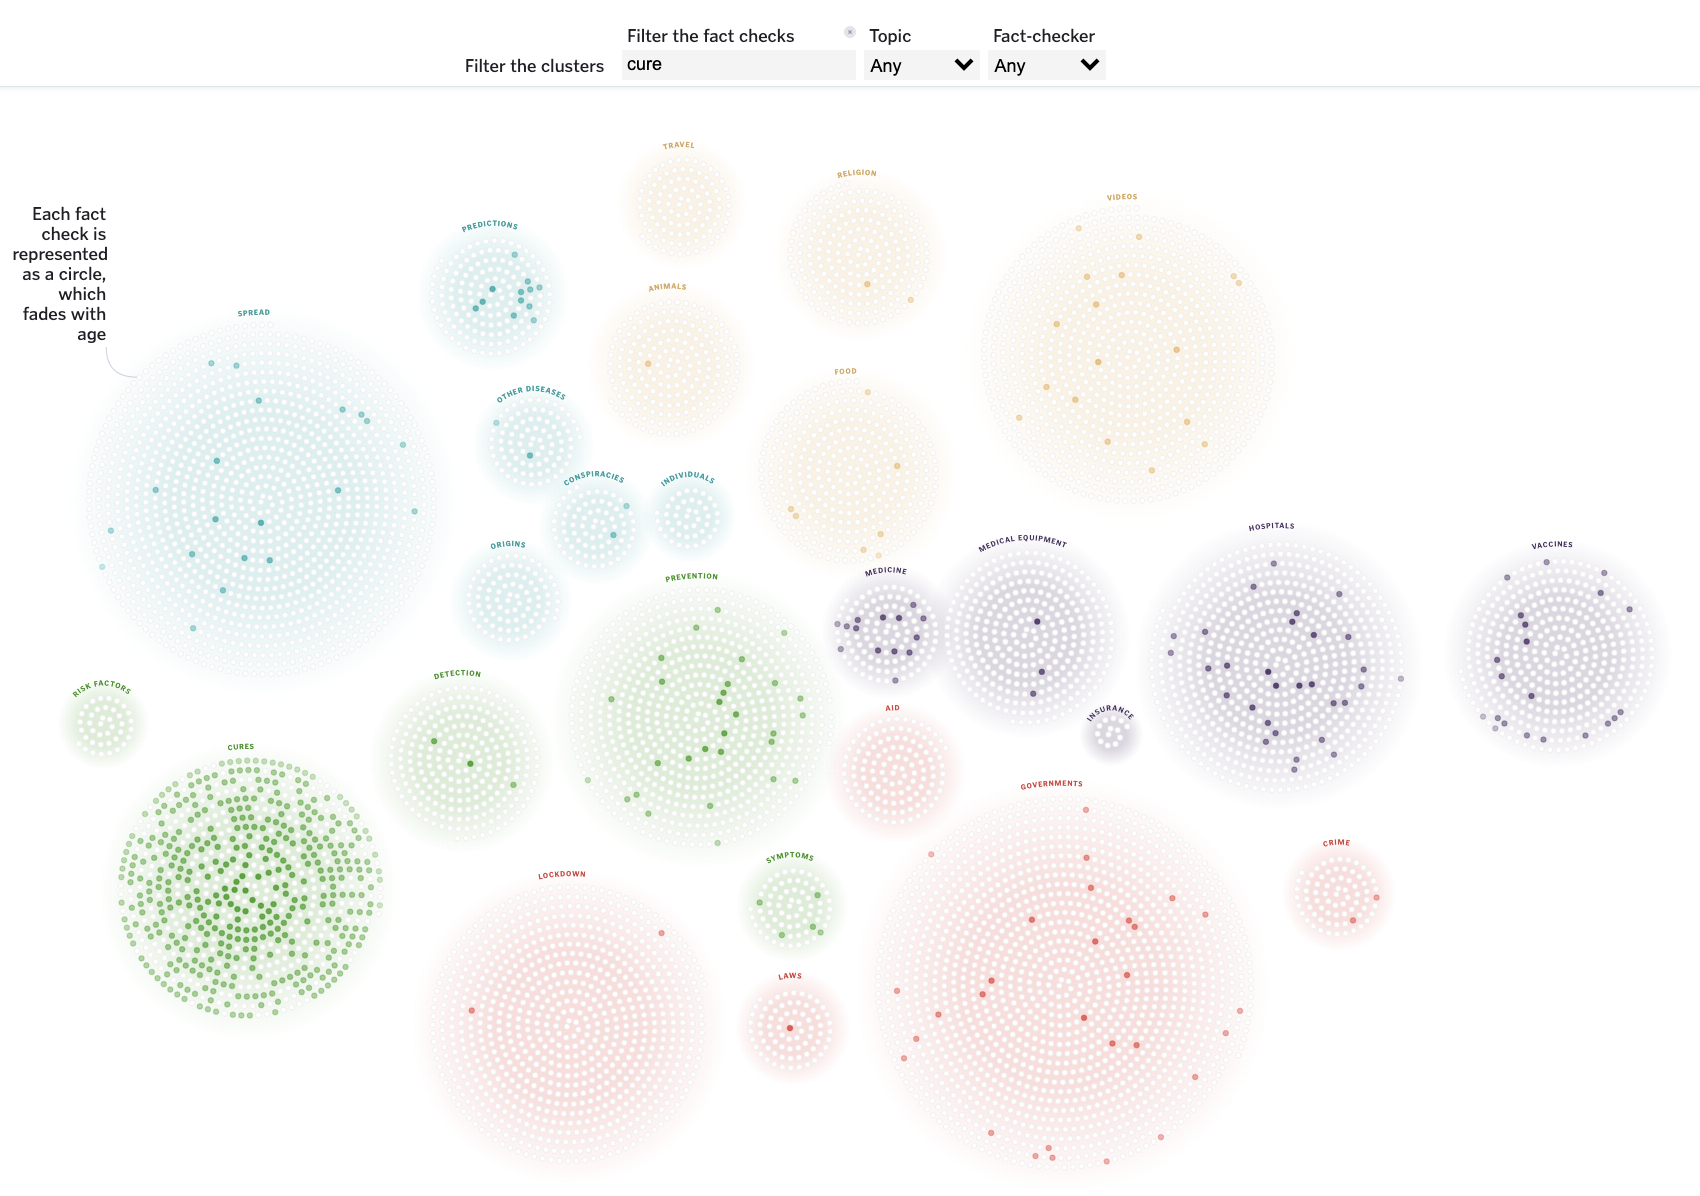
\includegraphics[width=.95\textwidth]{poynter_cures.png} 
\end{figure}
% https://www.poynter.org/coronavirusfactsalliance/


\FloatBarrier
\section{Experimental Setup}



\subsection{Sample recruitment}
We will recruit respondents in Kenya and Nigeria using Facebook advertisements targeted to users 18 years and older living in these countries.\footnote{Based on previous work it is clear that Facebook imputes location information for some of its users, which can be inaccurate \citep{Rosenzweig_2020}. We will also ask a location screening question to ensure our respondents live in our countries of interest.} %
To achieve balance on gender within our sample we create separate ads targeting men and women in both countries. Our target sample size is 1,500 respondents in each country for our pilot. Size of the full scale study will be determined following piloting, in procedures described in Section~\ref{simulations}. We anticipate that our sample will look similar to the overall Facebook population in these countries, which tends to be more male, more urban, and more educated than the overall population \citep{Rosenzweig_2020}. We will analyze how our sample compares to both the Facebook population and the general population in Kenya and Nigeria using Facebook's advertising API data and the nationally representative Afrobarometer survey that is conducted in both countries. 


Advertisements will appear within Facebook or Instagram, offering users with the opportunity to ``Take a 20 minute academic survey on Messenger - receive airtime.'' Incentives will be approximately 0.50-0.55 USD, accounting for transaction and messaging fees on the \href{https://africastalking.com/}{Africa's Talking} airtime distribution platform.%
\footnote{The recruitment advertisement is shown in Figure~\ref{fig:ad} in Appendix~\ref{appendix:recruitment}.} %
 When users click on the ``Send Message'' button on our advertisement, a Messenger conversation will open with our Facebook page, starting a conversation with a chatbot programmed to implement the survey.%
 \footnote{See Figure \ref{fig:chatbot} in Appendix~\ref{appendix:recruitment}.} % 
 In contrast to sending users to an external survey platform such as Qualtrics, the benefit of the chatbot is that we keep users on the Facebook platform, with which they are likely more familiar, and maintain a realistic setting in which users might encounter online misinformation.  Respondents who complete the survey in the chatbot will receive compensation in the form of mobile phone airtime sent to their phone. %%MOW: confirm survey completion time--and update advertisement accordingly




\subsection{Treatment}
Drawing on the literature on experimental interventions to combat misinformation, we include several interventions designed to reduce the spread of misinformation online, which are targeted both at the respondent level and headline level. This list of treatments also draws on real-world interventions that companies and platforms have instituted to combat misinformation. Treatments are presented in Table~\ref{tab:treatments}. 

% interesting point to maybe incorporate: Facebook, 24% of false-rated content in our sample remains up without warning labels \citep{brennen2020types}

\begin{table}[H]
\begin{tabular}{l|l|l}
\multicolumn{1}{c|}{\textbf{\begin{tabular}[c]{@{}c@{}}Shorthand\\ Name\end{tabular}}} & \multicolumn{1}{c|}{\textbf{\begin{tabular}[c]{@{}c@{}}Treatment\\ Level\end{tabular}}} & \textbf{Treatment}                                                                                                                                                                                                                                                                                                                                                                                              \\ \hline
Facebook tips                                                                                                           & Respondent                                                                                                   &  Facebook's ``Tips to Spot False News'' 
\\
AfricaCheck tips                                                                                                         & Respondent                                                                                                   &  \url{Africacheck.org}'s guide: \\ & & ``How to vet information during a pandemic''                                                                                                                                                                                                                                                                                                                             \\
Video training                                                                                                     & Respondent                                                                                                   &  \href{https://www.bbc.com/news/av/embed/p088bh96/52118949}{BBC Video training}                                                                                                                                                                                                                                                                                                                                                                                  \\
Emotion suppression                                                                                                       & Respondent                                                                                                   & \begin{tabular}[t]{@{}l@{}}Prompt: ``As you view and read the headlines, if you have any \\feelings, please try your best not to let those feelings show.  \\Read all of the headlines carefully, but try to behave so that \\someone watching you would not know that you are feeling\\ anything at all” \citep{gross1998emerging}.\end{tabular}
\\
Pledge                                                                                 & Respondent                                                                                                   &  \begin{tabular}[t]{@{}l@{}} Prompt: Respondents will be asked if they want to keep their\\ family and friends safe from COVID-19, if they knew \\COVID-19 misinformation can be dangerous, and if they're\\ willing to take either a \textit{private} or \textit{public} pledge to help identify\\and call out COVID-19 misinformation online (see \ref{sec:pledge}).
\end{tabular}
\\
Accuracy nudge                                                                                 & Respondent                                                                                                   & Placebo headline: ``To the best of your knowledge, is this\\& &headline accurate?'' \citep{pennycook2020fighting, pennycook_epstein_mosleh_arechar_eckles_rand_2019}.
\\
Deliberation nudge                                                                                 & Respondent                                                                                                   & Placebo headline: ``In a few words, please say \textit{why} you would\\ & & like to share or why you would not like to share this headline.''\\ & & [open text response]
\\
%Context                                                                                                        & Headline                                                                                                     & \begin{tabular}[t]{@{}l@{}}Facebook context button; if you click the info button on an\\ article, a pop-up tells you a few facts about the source: \\ how long the Facebook page has been registered,\\ and has a flag if article is more than 90 days old\end{tabular}
%\\
%Flag                                                                                                           & Headline                                                                                                     &  ``Disputed" flag on the headline                                                                                                                                                                                                                                                                                                                                                     \\
Related articles                                                                                                       & Headline                                                                                                     & Facebook-style related stories: below story,\\ & & show one other story which corrects a false news story                                                                                                                                                                                                                                                                                             \\
Factcheck                                                                                                      & Headline                                                                                                     & Fact checking flag from third party\\ & & (e.g., Facebook, AFP, AfricaCheck, etc)
 \\
More information                                                                                                      & Headline                                                                                                     & Provides a link to ``Get the facts about COVID-19''\\ & & as per Twitter flags
 \\
 Real information                                                                                                      & Headline                                                                                                     & Provides a \textit{true} statement: ``According to the WHO,\\ & & there is currently \textbf{no proven} cure for COVID-19.
 \\
Control                                                                                                        & N/A                                                                                                          & Control condition                                                                                                                                                                                                                                                                                                                                                                                              
\end{tabular}
\caption{Description of interventions included in the experiment}
\label{tab:treatments}
\end{table}

Respondent-level treatments and headline-level treatments are implemented as separate factors, each of which has an empty baseline level that is the control. So respondents may be assigned the pure control condition, one of the respondent-level treatments but no headline-level treatment, one of the headline level treatments but no respondent-level treatment, or one of the respondent-level treatments \textit{and} one of the headline-level treatments. 


%\textbf{MORE on why these treatments:}
%1. Guess et al - forthcoming - who find that FB tips for spotting fake news improved discernment in the US + India (Nyhan 2020, p.231)
%2. nigeria data suggest correlation between feeling sad and afraid with improved discernment between true/false stimuli and associated with greater sharing intentions of true (more than false) stimuli -- but other work from US (non-covid) suggests emotion regulation can help improve discernment -- 
% Feeling happy and experiencing cognitive ease provides people with a signal that everything is going well—and it leads them to rely on their intuition. Feeling sad or experiencing metacognitive difficulty, in contrast, signals that everything is not going well. This can trigger the motivation to be more careful and deliberate (Alter, Oppenheimer, Epley, & Eyre, 2007; Bless, Schwarz, & Wieland, 1996; Isen, Nygren, & Ashby, 1988, but see Meyer et al., 2015 and Thompson et al., 2013).


\subsection{Covariates}

Covariate measurement plays an important role in our contextual adaptive experiment. We assign treatment conditional on context, where the context is defined by the measured pre-treatment covariates. (Procedures for treatment assignment are detailed in Section ~\ref{adaptiveagent}.)
The motivation for this \textit{contextual} adaptive experiment comes from the widely shared belief by misinformation scholars that \textit{context matters.} More specifically, scholars note that ``...not all misinformation is created equal, nor are all individuals equally susceptible to its influence'' \citep{wittenberg2020misinformation}. In addition to heterogeneity in individual's susceptibility to misinformation ``responses to corrections are likely heterogeneous'' \citep{swire2020searching}. Hence, we expect to observe heterogeneity in the effectiveness of the treatments described in the previous section and explicitly incorporate this into our experimental design by pre-specifying the covariates that we anticipate to moderate treatment effects.

Despite the fact that many prominent scholars emphasize the importance of context and heterogeneity among individuals, misinformation research generally treats heterogeneous treatment effects as secondary analyses. In the existing misinformation literature, centered around studies conducted with respondents in the North America and Europe, the covariates of interest include political ideology \citep{pennycook_epstein_mosleh_arechar_eckles_rand_2019}, cognition or inclination to deliberate \citep{bago2020fake}, and media literacy \citep{guess2020digital}.  

This project expands this focus to explore heterogeneity with respect to additional respondent covariates. Outside of contexts where partisanship is a salient identity and lens through which individuals interpret news and information, what are the likely sources of heterogeneity in individual's receptivity to interventions to combat the spread of misinformation? We highlight several key covariates that we predict will inform the effectiveness/suitability of our interventions for individuals with respect to countering the spread of COVID-19 misinformation. 


In addition to the demographic covariates commonly used in social science research, we also include specific questions regarding knoweldge of and concern about COVID-19, an index of scientific views, beliefs about government efficacy in the current coronavirus pandemic, religious behaviors and beliefs, locus of control, and digital literacy. The full list of covariates and question wording is in Appendix~\ref{appendix:covariates}. These variables capture what other researchers have suggested are primary sources of heterogeneity in responses to misinformation: age, analytical thinking (captured in our scientific beliefs index), and need for closure (captured in our concern regarding COVID-19 concern measurement and the beliefs about government efficacy measurement) \citep{wittenberg2020misinformation}. 



%\textcolor{red}{EDITING...Psychological need for control + uncertainty of pandemic → superstitious beliefs / magical thinking
%Locus of control is defined as ``a generalized attitude, belief, or expectancy regarding the nature of the causal relationship between one's own behavior and its consequences'' (Rotter, 1966).
% An individual with an internal locus of control will ``attribute outcomes to their own actions'' while an individual with an external locus of control will attribute it ``to circumstances beyond their control'' (Rotter, 1966).
%Understand differences in effort/motivation
%More internal locus of control associated with higher education/income
%Health outcomes (cite psych paper)
%}

% Several of our treatments also target these features, such as analytic thinking (the deliberation and emotion suppression treatments).  




\textbf{Predictions about covariates/heterogeneity:}\todo{@Molly do you think we should include this kind of thing here?}\todo{@Leah, I would if anything put a few of these in a paragraph form, and say, "However, our objective is to learn an optimal policy conditional on covariates, and not to determine which covariates matter, and by how much. For this reason, we refrain from formalizing hypotheses regarding treatment effect heterogeneity." What do you think?}
\textcolor{red}{
\begin{enumerate}
\item At a high level, we expect to see results such as individuals with low digital media literacy will be most affected by the respondent-level false news video training combined with the factcheck headline treatment. Younger respondents who have a high level of concern about COVID-19 will be most affected by the pledge treatment combined with the related articles or factcheck headline treatments.
\item Individuals who are more literate with respect to digital media will be most affected by the headline-level treatments. We also expect more educated and less religious individuals to be more influenced by these treatments.
\item More educated and less religious individuals will be less influenced by our accuracy nudge or deliberation nudge treatments.
\item Emotion suppression and accuracy nudge treatments will be more effective for low CRT and older respondents.
\item Contrary to existing research based in the US, we do not expect partisanship to interact with our treatments.
\item Sides 2016 + Gilens 2001 (information treatment more effective on high knowledge ppl)
\item we expect that religiosity and religious beliefs - as well as locus of control - to matter...
\item in US social distancing measures adopted at higher rates in areas with more climate change believers %https://www.researchgate.net/profile/David_Van_Dijcke/publication/341001499_Belief_in_Science_Influences_Physical_Distancing_in_Response_to_COVID-19_Lockdown_Policies/links/5ea96a1e92851cb267633a3d/Belief-in-Science-Influences-Physical-Distancing-in-Response-to-COVID-19-Lockdown-Policies.pdf
\end{enumerate}
}

% - include more covariates in the pilot and then subset for actual survey
%	- include a couple different measures of covariates



\subsection{Outcomes and Response Function}

We are interested in decreasing sharing of harmful false information about COVID-19 cures and treatments while not negatively impacting sharing of useful information about transmission and best practices from verified sources. Specifically, we are interested in three outcomes: (1) Self-reported intention to share a given story, (2) Actual behavior with respect to sharing that story\footnote{Though this is only measured for the \textit{true} headlines as respondents are mostly prevented from sharing the falsehoods.}, (3) Willingness to share tips and information about misinformation more generally. For all reported outcomes and responses (excluding aggregated tallies discussed below), analysis will be conducted as described in Section~\ref{analysis}.  

\subsubsection{Primary Response Function}

We measure interest in sharing information through two questions:
\begin{itemize}
\item Would you like to share this post on your timeline? 
\item Would you like to send this post to a friend on Messenger?
\end{itemize}

Prior to treatment, we show respondents two articles from their country randomly sourced from our misinformation stimuli and two articles randomly sourced from our true information stimuli, in random order, and for each stimuli we ask the above self-reported interest questions. Respondents are then asked a series of unrelated questions, and are then randomly assigned treatment according to the experimental design. If assigned one of the respondent-level treatments, they are administered the relevant treatment. They are then shown two additional misinformation stimuli and two additional true information stimuli, selected from the remaining stimuli that they were \textit{not} shown pre-treatment. If the respondent is assigned a headline-level treatment, this treatment is applied only to the misinformation stimuli, as flags and fact-checking labels are not generally applied to true information from verified sources.\footnote{The initial implementation of Twitter's labeling of coronavirus-related tweets with links to additional information was deemed to be overly broad, and was applied to some tweets that did not include misinformation. Twitter revised their labeling in late June of 2020. A company message was released on June 26: \url{https://twitter.com/TwitterSupport/status/1276661483561029632}. } For each of the stimuli we again ask the same self-reported sharing intention questions. 

By using a pre-test / post-test design  \citep{davidian2005semiparametric} %https://declaredesign.org/library/articles/pretest_posttest.html
and an index of repeated measures \citep{broockman2017design}, we aim to improve the efficiency of our effect estimation. 


We code response to the self-reported interest questions as 1 if the respondent affirms and 0 otherwise. Let $M_i^1$ be the sum of respondent $i$'s pre-test responses to the \textit{misinformation} stimuli and let $T_i^1$ be the sum of respondent $i$'s pre-test responses to the \textit{true} informational stimuli. $M_i^2$ and $T_i^2$ are the respective post-treatment responses. Then $M_i^1, T_i^1, M_i^2, T_i^2 \in {0,1,2, 3, 4}$. 

We control for strata of pre-test responses in our analyses, i.e., $S=\{(m^1, r^1)\in M^1 \times R^1\}$. 
We formalize our response function in terms of post-test measures:
\[
Y_i = -M^2_i + 0.5 T^2_i.
\]
This response function will be the metric that we optimize for in our adaptive algorithm described in Section~\ref{adaptiveagent}, and in our policy learning described in Section~\ref{analysis}. Because of random assignment, we expect to see no systematic differences in pre-test interest in sharing either true or untrue stimuli across treatment conditions, conditional on covariates. %For a given treatment condition, all else equal, if respondents share misinformation at lower rates post-test compared to control, this will result in a relatively higher response variable. If respondents share true information at lower rates post-test compared to control, this will result in a relatively lower response variable, but the relative impacts are only half as large as those for the misinformation stimuli. 




\subsubsection{Secondary Outcomes}
Additionally, we measure secondary behavioral outcomes which allows us to further investigate the extent to which treatments may suppress the sharing of \textit{true} information.

In order to obtain a behavioral measure of sharing, we collect the articles the respondent indicated they would like to share throughout the survey and at the end of the survey provide links to the \textit{true} information. For these true stimuli, we offer respondents the opportunity to actually share this information as a Facebook post, which has been created on our project Facebook page. We are able to measure whether respondents click on a button which opens a pop-up screen to share the post on Facebook, however, we cannot measure directly whether they then actually follow through to the second step and post the article on their own timeline. Consequently, we report only rates of clicking the initial share button. The response function here is measured as the percent of true stimili that the respondent said they wanted to share during the survey for which they later click the button to share on Facebook. (We do not differentiate between stimuli presented pre- and post- treatment here, since the behavioral response measurement for all stimuli is all post-treatment.) To provide some insight on the extent to which respondents followed up on an intention to share, we report the \textit{aggregate} number of times the associated post for each stimuli was shared. %We \textit{could} actually create a separate post for each treatment combination, and measure sharing that way, but this seems like overkill for a secondary outcome in an already complicated project.

At this point we also debrief respondents, informing them about the headlines they were shown that are false. Instead of allowing respondents to share these headlines, we provide links to tips for spotting misinformation online and also offer them the opportunity to share these tips on their timeline or on messenger; we measure intention to share these tips and aggregate number of shares of tips by treatment condition as well. 


\subsubsection{Attrition} We will include in analysis all respondents for whom we have collected complete pre-test responses. As treatment is not revealed at this point, attrition should be independent of treatment assignment conditional on covariates. For respondents who attrit after collection of pre-test responses and before collection of post-test responses, all types of post-test responses will be coded as zero.\footnote{An alternative approach to analysis in a pre-test/post-test design, accounting for missing data, would be to follow \cite{davidian2005semiparametric}'s implementation of estimators developed by \cite{robins1994estimation}.}


\section{Hypotheses and Data Collection}



Our data is described by treatments $W_i \in \ww$\footnote{Our treatments are composed of two separate factors, but here we use $W$ to represent combined treatment conditions, i.e., the unique combination of one respondent-level and one headline-level treatment. Where we wish to explicitly differentiate, we use $W^R_i$ and $W^H_i$ for respondent- and headline-level treatments respectively. Each factor includes a baseline level absent intervention, and the cardinality $|\ww| = |\ww^H|\times |\ww^R|$.}; response,  $Y_i \in \RR$; and covariates, $X_i \in \xx$. 

We assume the data is indexed by $i = 1, \dots, N$ where indexing represents the order in which respondents entered the experiment; this allows us to use $i$ to also represent relative chronological relationships in our sequential adaptive design. 

We use potential outcome notation, where $Y_i(w)$ represents the potential outcome for respondent $i$ under treatment $w$.%, and by experimental design,  we have strong ignorability of potential outcomes to treatment conditional on observed covariates. 


We would like to learn and evaluate an optimal contextual policy, under which we assign the most effective treatment conditional on covariates. Formally, a policy maps a set of covariates to a decision \citep{athey2017efficient}, %\todo{Update reference}
\begin{align}
  \pi: \xx \rightarrow \ww. 
  \label{eq:policy}
\end{align}
In our setting, we will learn this policy, $\hat \pi$, and evaluate its value. The value of a policy is defined as, 
\begin{align}
V(\pi) =  \E[Y(\pi(X_{i}))],
  \label{eq:policy_value}
\end{align}
where the expectation is taken over the distribution of $X$.\footnote{Here we will only consider deterministic policies, but for a random policy, the expectation will be taken over the joint distribution. }

\subsection{Hypotheses}\label{hypotheses}

Our hypotheses of interest relate the value of an estimated optimal contextual policy $\pi_{opt}$ to fixed policies $\pi_{W}$, where under each fixed policy we would assign all respondents the relevant treatment $w$. The control policy is the fixed policy $\pi_{w_{C}}$

Our primary hypothesis is that we are able to estimate from the data an optimal contextual policy that improves over the control. 
  \begin{hypothesis}
  The best contextual policy that can be estimated from the data achieves higher value than the control treatment \label{eq:optctr}.
\begin{align}
  H_{0}: V(\pi_{opt}) = V(\pi_{w_{C}}) \qquad H_{a}:  V(\pi_{opt}) > V(\pi_{w_{C}})
\end{align}
\end{hypothesis}
This is the hypothesis that we aim to optimize power for in our adaptive data collection. 

We would also like to learn how much we gain by exploiting heterogeneity in the data. As a secondary hypothesis, we propose that the optimal policy that we are able to estimate from the data improves over the best fixed policy. 
  \begin{hypothesis}
  The best contextual policy that can be estimated from the data achieves higher value than the best fixed policy, i.e., the fixed policy with the highest associated value. 
  \label{eq:optmax}
\begin{align}
  H_{0}: V(\pi_{opt}) = \argmax_w V(\pi_{w}) \qquad H_{a}:  V(\pi_{opt}) > \argmax_w V(\pi_{w})
\end{align}
\end{hypothesis}


\subsection{Adaptive data collection}\label{adaptiveagent}

To collect data with the objective of learning an optimal policy, we use a \textit{contextual bandit} algorithm, in which we sequentially update treatment assignment probabilities based on the observed history of treatments, response, and covariates. These types of algorithms navigate a tradeoff in \textit{exploration} of the treatment space with \textit{exploitation} of those treatments which we have observed to be effective based on historical data. This allows us to continue to learn about treatment effect heterogeneity while continuing to improve outcomes over time \textit{within} the frame of the experiment. 

We will use a version of linear Thompson sampling \citep{agrawal2013thompson}. Under Thompson sampling \citep{thompson1933likelihood,thompson1935theory}, treatment is assigned according to the Bayesian posterior probability that each treatment is best. In linear Thompson sampling, this is generalized to allow the outcome to be a linear function of covariates. Under this approach, we assume there is some unknown coefficient vector $\theta_w\in R^{|\xx|}$ for each arm $w \in \ww$, such that $Y_i(w) = x_i^\top \theta_w + \epsilon_i$, and $\epsilon_i\sim \mathcal{N}(0, \sigma_w)$, i.e., variance is constant under each arm. The conditional mean is $\mu_w(x) = \E[Y(w)|X=x] = x^T \theta_w$. 

%We assume the variance is constant within arms, i.e., $\V[Y(w)|X = x] = \sigma^2_w$. The conditional reward function is modeled as being distributed,
%  \begin{align}
%    \mu_w(x) \sim \mathcal{N}({\mu}_w(x), {\sigma}_w^{2}(x)) \qquad %\text{for } s \in \{1, \cdots, S\} \text{ and treatment }w
%    \text{ for all treatments }w \in \ww
%  \end{align}


Our implementation closely follows the balanced linear Thompson sampling algorithm described in \cite{dimakopoulou2017estimation, dimakopoulou2019balanced}, where the estimates $\hat\theta_w$ and $\hat\sigma^2_w$ are produced using weights to account for unequal assignment probabilities. We use a batched approach to updating, collecting data in batches and then updating treatment assignment model after each batch. We denote batches $\mathcal{I}_b$ for $b = 1, \dots, B$. Full details for the algorithm are provided in Algorithm~\ref{algg:bblts}, we present an overview below. 

\paragraph{Adaptive agent}\todo{This needs to be tweaked slightly to match Algorithm~\ref{algg:bblts}. }

\begin{enumerate}
\item In the first batch, $b = 1$, we assign treatment uniformly at random. 

\item For equally sized batches $b = 2, \dots, B-1$:

\begin{enumerate}
   \item \label{step:fit} Fit a ridge regression with balancing weights. Compute the minimum mean cross-validated error value of the penalization factor $\lambda^{CV}$ using the entire observed history of data.%
 \footnote{We set M = $1,000$.}
 \footnote{For the agent we use a linear model, with treatment indicators, covariates, and treatment and covariates interacted:
 
%\begin{align*}
%\hat{\mu}_w(X_{i}) & =
%			\sum_{w^R} 1\{W^R_i = w^R\}\hat\beta_{w^R}  +
%			\sum_{w^H} 1\{W^H_i = w^H\}\hat\beta_{w^H}  +\\ 
%			& \sum_{w^R} \sum_{w^H}1\{W^R_i = w^R\} \times 1\{W^H_i =  w^H\}\hat\beta_{w^{R,H}} +  \\
%			& \sum_{\ell}  X_{[\ell]i}\hat{\beta}_{\ell} +\\
%			& \sum_{w^R} \sum_{w^H}1\{W^R_i = w^R\} \times 1\{W^H_i =  w^H\}  X_{[\ell]i} \hat{\beta}_{w^{R,H}, \ell}.\numberthis
%         \label{eq:linear_model_full}
%\end{align*} 

\begin{align*}
\hat{\mu}_w(X_{i}) & =
			\sum_{w} 1\{W_i = w\}\hat\beta_{w}  +
			\sum_{\ell}  X_{[\ell]i}\hat{\beta}_{\ell} +
			\sum_{\ell} \sum_{w}1\{W_i =  w\}  X_{[\ell]i} \hat{\beta}_{w, \ell}.\numberthis
         \label{eq:linear_model_full}
\end{align*} 

%The model is estimated using $L_{2}$ penalties for regularization, exclusive of the main treatment effects $\beta_{w^R}$ and $\beta_{w^R}$ and interaction of treatment levels, $\beta_{w^{R,H}}$. 
The model is estimated using $L_{2}$ penalties for regularization, exclusive of the main treatment effects $\beta_{w}$. 
Observations are weighted according to inverse probability weights using known assignment probabilities, following \cite{dimakopoulou2017estimation}, as in Equation~(\ref{eq:IPW}) in Appendix~\ref{appendix:stabilized}. %Stabilized inverse probability weights are discussed in Appendix~\ref{appendix:stabilized}. 
}
  
  
 This model with penalty factor $\lambda^{CV}$ produces our estimate of the coefficient vector $\hat \theta_w$ and an associated estimated variance, $\V[\hat\theta_{w}] $ for each arm $w\in \ww$ . 

 \item For each observation, we draw $M$ draws from $\tilde \theta ^{(m)}_w \sim \mathcal{N}(\hat \theta_w),\V[\hat\theta_{w}]$ for each condition $w$, and calculate the proportion of times each arm produced the maximum estimate under the covariate profile $x_i$:\footnote{Note that we slightly abuse notation here, as for each $ x_i^\top \tilde \theta ^{(m)}_w$ the $x_i$ term is modified to the appropriate format for relevant treatment indicators and interactions for each hypothetical treatment $w$. I.e., we are producing predictions given the observed covariates under each counterfactual treatment condition. }
				\begin{align}
    q_w(X_i) = \frac{1}{M} \sum_{m=1}^M 1\left\{ w = \argmax_w \{ x_i^\top \tilde \theta ^{(m)}_1, \dots, x_i^\top\tilde \theta_{|\ww|}^{(m)} \}  \right\}.
				\end{align}
\item Denote the control condition $w_{C}$, and assign a fixed probability $1/|\ww|$ to the pure control condition, i.e., $\tilde{q}_{w_C} = 1/|\ww|$. For the remaining probabilities given each possible context $x$, update assignment probabilities so that they sum to 1, constraining the minimum assignment probability to a pre-determined probability floor, $p$
      \begin{align}
          \tilde{q}_w(X_i) & =\max\Biggr\{\frac{ q_{i}(w)}{\sum\limits_{w \neq w_{C}}q_{i}(w) } , p\Biggr\} \\
          e_{w}(X_i) & = \frac{ \tilde{q}_w(X_i)}{\sum\limits_{w \neq w_{C}}\tilde{q}_w(X_i) }. 
      \end{align}
\item Assign treatment  according to the calculated probabilities: $w_i \sim \textrm{Multinom}(\tilde{q}_{i}(1), \dots, \tilde{q}_{i}(|\ww|))$
\end{enumerate}

\item For the final batch,  $b = $ B, collect data on-policy:
\begin{enumerate}
  \item Estimate conditional means by fitting a random forest estimator on the entire data set collected through batch $B-1$, following the steps outlined in Appendix~\ref{appendix:grf}, adjusting for adaptively collected data as described in Appendix~\ref{appendix:DRlfo}. 
%  Here, we can use the full covariate set, as described in Appendix~\ref{appendix:covariates}.
  \item Fit a point-wise optimal policy  by taking the maximum of predicted values for each possible context $x$ 
    \begin{equation}
     \hat{\pi}_{x} = \argmax_{ w } \hat{\mu}_{w}(x) . 
    \end{equation} 
  Store the policy. 
  \item Collect data for the batch: For every new respondent, collect data on their contexts, and assign treatment deterministically consistent with $\hat{\pi}_{x}$. 
\end{enumerate}
\end{enumerate}


\section{Analysis}\label{analysis}

To estimate the value of a policy, we take the average of doubly robust scores $\Gamma_{i,w}$, as in (\ref{eq:DR}), following \cite{robins1994estimation}'s augmented inverse-propensity weighted scores, 

      \begin{align*}
        \Gamma_{i,w} = \mu_{w}(X_{i}) + 1 \{W_i = w \} \gamma_w(X_i)(Y_{i} - \mu_w(X_i)). \numberthis\label{eq:DR}\\
         \mu_{w}(x)  = \E[Y_i(w) | X_i = x]
    \end{align*}

We will estimate $\hat\mu_{w}(X_{i})$ for each $w$ using generalized random forests, following the approach is described in Appendix~\ref{appendix:grf}. $\xi_w(X_i)$ is a weight to account for unequal treatment assignment probabilities; we may use inverse probability weights calculated from the actual probabilities assigned under the experimental design; in practice, we use the stabilized versions of these weights, as described in Appendix~\ref{appendix:stabilized}.  Again, we can use the full covariate set, as described in Appendix~\ref{appendix:covariates}, including the pre-test response measures on the righthand side of the model.

Our methods for analysis will differ depending on how the data is collected. 

\subsection{Policy learning and evaluation on randomly collected data}\label{randomlearning}
For randomly collected data, as in the pilot, we conduct policy learning and evaluation as below:

\begin{enumerate}
  \item Collect data by assigning treatment uniformly at random.
  \item Estimate nuisance components $\hat{\mu}_{w}(X_i)$ for each treatment separately, following the steps detailed in Appendix~\ref{appendix:grf}; for  $\hat\xi_w(X_i)$, use assigned probabilities $1/|\ww|$. 
  \item Compute doubly robust scores $\hat{\Gamma}_{i,w}$ substituting the estimated nuisance components into (\ref{eq:DR}). 
  \item Fit a point-wise optimal contextual policy $\hat{\pi}_{opt}$ by taking the maximum of predicted values at each point
    \begin{equation*}
\hat{\pi}_{x_i}  =     \argmax_{w} \hat{\mu}_{w}(x_i) 
    \end{equation*}
  \item To evaluate the policies, take the average scores :
    \begin{align*}
          \hat{V}({\pi}_{w})  &:= \frac{1}{N} \sum_{i}^N \hat{\Gamma}_{i,w} \\
      \hat{V}(\hat{\pi}_{opt})  &:= \frac{1}{N} \sum_{i}^N \hat{\Gamma}_{i, \hat{\pi}_{X_i}} 
          \end{align*}
   \item To learn and evaluate the best fixed policy on a dataset, we cannot simply take the treatment condition with the highest estimated value, as this will give us positive bias in expectation. To account for this, we use the approach described in Appendix~\ref{appendix:bestfixed}. 
\end{enumerate}


\subsection{Policy learning and evaluation on adaptively collected data}\label{adaptiveearning}
For adaptively collected data, as in the simulations discussed in Section~\ref{simulations} and our eventual experiment, we conduct policy learning and evaluation as below:

\begin{enumerate}
\item Collect data under the adaptive algorithm described in Section~\ref{adaptiveagent}. 
\item For our nuisance components, due to the dependent nature of the data, we must ensure that our estimation is conducted using only historical data. Estimate nuisance components $\hat{\mu}_{w}(X_i)$  and $\hat\xi_w(X_i)$ for data up to and including batch $B-1$ following the steps outlined in Appendix~\ref{appendix:DRlfo}. 
\item Compute doubly robust scores $\hat{\Gamma}_{i,w}$ substituting the estimated nuisance components into (\ref{eq:DR}). 
\item We have already fitted and stored a point-wise optimal policy to conduct the on-policy evaluation in the final batch $B$ of the adaptive experiment. 
  \item To evaluate the policies, we take the average scores over the relevant evaluation sets $\mathcal{I}$, where $\mathcal{I}_b$ represents the set of all observations within batch $b$. We note that evaluation of the optimal policy is simplified, due to the on-policy evaluation in the final batch $B$:
      \begin{align}
          \hat{V}({\pi}_{w})  &:= \frac{1}{\bigg{\lvert} \bigcup\limits_{b=1}^{B-1} \mathcal{I}_{b} \bigg{\rvert}} \sum_{i \in \bigcup\limits_{b=1}^{B-1} \mathcal{I}_{b} } \hat{\Gamma}_{i,w} \\
                     \hat{V}(\hat{\pi}_{opt})  &:= \frac{1}{\big{\lvert}  \mathcal{I}_{B} \big{\rvert}} \sum_{i \in \mathcal{I}_{B} }
                      Y_i  
    \end{align}
   \item To learn and evaluate the best fixed policy on a dataset, we again take the relevant approach described in Appendix~\ref{appendix:bestfixed}. 
\end{enumerate}

To evaluate the hypotheses from Section~\ref{hypotheses}, we estimate standard errors using the standard deviations of the relevant scores, and conduct frequentist hypothesis testing. 

The data collected from this study may be used for eventual application of a contextual implementation of the evaluation weighting method proposed in \cite{hadad2019confidence}, and advanced for contextual cases in \cite{zhan2020retrospective}. However, these methods will not be discussed in this pre-registration. 



\subsection{Simulations and design parameters}\label{simulations}

\textit{\textbf{Note:} This section provides an overview of our approach to making data-driven design decisions. We will update this pre-analysis plan \textit{after} collecting pilot data and running simulations, to document simulation results and our final design parameters, prior to implementing the eventual adaptive experiments. }

To carry out implementation, the above description requires setting of several design parameters, including total experiment size $N$, number of batches $B$,  size of first batch $|\mathcal{I}_1|$, size of last batch $|\mathcal{I}_B|$, and probability floor $p$. 

We set these parameters by learning from our pilot data of 1500 observations from each country. In the pilot data, treatment is assigned uniformly at random. We conduct the below simulations \textit{separately} for each country, meaning that we may end up with meaningfully different designs in the two countries. 

We then simulate data generating processes (DGPs) based on the pilot data, with varying heterogeneity. We create these DGPs by fitting a model to each dataset following (\ref{eq:linear_model_full}) and using covariates in Appendix~\ref{appendix:covariates}, but instead of learning and applying the cross-validated penalty factor $\lambda^{CV}$, we generate models with varying complexity by over- and under-fitting to the data, imposing different penalty factors. In ridge regression, larger penalties will be associated with more parsimonious models, and less heterogeneity. Smaller penalties will be associated with more complex models, and consequently more heterogeneity. This approach allows us to generate heterogeneity that would plausibly exist in the true underlying populations. 

We refer to the heterogeneity ``ratio'' as the ratio of the value of the best contextual policy over the value of the best fixed policy. A ratio of two would indicate that the best contextual policy returns response that is in expectation twice as large as response under the best fixed policy. We can create a DGP with no heterogeneity by setting an arbitrarily large penalty factor, shrinking all treatment $\times$ covariate interactions to (effectively) zero. 


\paragraph{Data generating processes}
\begin{enumerate}
%\item Define a vector of potential $\lambda$ values, \textcolor{red}{[TK, inclusive of zero]}. 
\item  Sample $S=10,000$ observations with replacement from the empirical distribution of covariates in the pilot data; store this as $X^{(1)}, \dots,X^{(S)}$. 
\item Estimate heterogeneity ratios under each element of the vector of penalty factors:
\begin{enumerate}
\item Fit the model (\ref{eq:linear_model_full}) to the pilot data under the relevant penalty factor to generate conditional means models $\mu_{w}(X)$ for each treatment $w$.
  \item Calculate conditional means $\mu_{w}(X^{(s)})$ under the above fitted model conditional on covariates $X^{(1)}, \dots,X^{(S)}$. 
  \item Estimate and store values for fixed policies for each $w$
      \begin{align}
          \hat{V}({\pi}_{w})  &:= \frac{1}{S} \sum_{s = 1}^S \mu_{w}(x^{(s)}) \\
          \end{align}
  \item Fit a point-wise optimal policy on the resampled data by taking the maximum conditional mean for each individual context $x^{(s)}$ 
    \begin{equation}
     \pi_{x^{(s)}} = \argmax_{ w } \mu_{w}(x^{(s)}) . 
    \end{equation} 
    \item Estimate and store value for the optimal policy:
    \begin{align}
      \hat{V}(\hat{\pi}_{opt})  &:= \frac{1}{M} \sum_m \hat{\mu}_{\hat{\pi}_{x^{(s)}}}(x^{(s)}) 
          \end{align}
  \item Estimate the heterogeneity ratio as $\hat{V}(\hat{\pi}_{opt})/\hat{V}(\hat{\pi}_{w_{max}})$, where $w_{max}$ is the true best arm under the relevant conditional means model over the empirical distribution of covariates. 
\end{enumerate}
\item Search over the vector of potential penalty factors to find:
\begin{enumerate}
\item The factor with an associated heterogeneity ratio that is closest in absolute distance to 1.05. This will allow us to learn about the performance of our algorithm in a case with a small amount of heterogeneity. 
\item The largest penalty factor within one standard deviation of cross validated error from no penalization. 
\item The two penalties factors which minimize the absolute distance to 1/3 and 2/3 of the distance between 1.05 and the above near-largest heterogeneity ratio. 
\end{enumerate}
\end{enumerate}

\paragraph{Simulations}
This then gives us four conditional mean models. We then generate data from these models by:
\begin{enumerate}
\item  Sampling covariates from the empirical distribution from the pilot data and assigning response as the conditional mean + a noise term, where the noise term is based on the mean error between the fitted model and the pilot data, estimated separately for each treatment. 
\item We run a series of simulated experiments using data from each of the DGPs, randomly applying parameters from Table~\ref{tab:design} so that we have 500 iterations of experiments run under each unique combination of design parameters for each DGP. 
\end{enumerate}


\paragraph{Parameter choice}
Our objective in selecting design parameters is to optimize power for Hypothesis~\ref{eq:optctr}, while minimizing the size of the experiment and the number of batches. From the simulations we should be able to learn about power conditional on each combination of design parameters. Our decision rule is as follows:
\begin{enumerate}
\item Estimate power for Hypothesis~\ref{eq:optctr} under each unique combination of design parameters for each DGP. Take the average power across DGPs, conditional on each unique set of design parameters. 
\item If there is one or fewer combinations of design parameters with average power $\ge.8$, select the set of design parameters which optimizes Hypothesis~\ref{eq:optctr}. To break ties, select the set with smallest experiment size, or, if of equal size, select with smallest number of batches. If experiment size and batch size are equal, select randomly. 
\item If there is more than one combination of design parameters with average power $\ge.8$, constrain choices to only those sets with average power $\ge.8$. Then constrain choices to only those sets with the smallest experiment size, and then to the smallest number of batches. Among the remaining sets, optimize for power of Hypothesis~\ref{eq:optctr}. To break ties, select randomly. 
\end{enumerate}

\begin{table}[H]
\centering
\caption{Design parameters} 
\label{tab:design}
\begin{tabular}{l | l}
\textbf{Parameter} & \textbf{Choice set} \\ \hline
Total experiment size ($N$)& [2500, 3750, 5000] \\
Number of batches ($B$)& [10, 15, 20] \\
First batch size ($|\mathcal{I}_1|$) & $N \times$ [1/10, 1/5, 3/10] \\
Last batch size ($|\mathcal{I}_B|$) &  $N \times$ [1/10, 1/5, 3/10] \\
%Outcome model & [Ridge, Random Forest] \\
%Balancing weights & [Batch-wise IPW, ARB]\\
Probability floor (p)& [0.05, 0.1, 0.25]$\times 1/ |\ww|$ \\
\hline
\end{tabular}
\end{table}


\section{Power Calculations}
The ensure the robustness of our adaptive design, we consider performance of our algorithm across a variety of simulated conditions. We assume there are three groups, and within each group, conditional on covariates, a different arm gives the highest reward. We then vary:
\begin{itemize}
\item \textbf{Relative size of the groups.} We allow the largest group to be 0.8, 0.6, and 0.4 of the underlying population, with the two remaining groups approximately equally sized
\item \textbf{Number of predictive covariates.} We vary the number of covariates used to predict group membership
\item \textbf{Heterogeneity ratio.} We vary the relative value of the best contextual policy to the best fixed policy to be 1.05, 1.5, or 1.95. 
\end{itemize}


\todo{Figures TK}

\clearpage
\bibliographystyle{apalike}
\bibliography{fb_misinfo_references}

\clearpage
\appendix

\section{Recruitment}\label{appendix:recruitment}
Respondents will be recruited through Facebook advertisements (Figure \ref{fig:ad}) that appear on their news feed, mobile application, and instagram. 

\begin{figure}[htb]
\centering
\caption{Advertisement as run in Facebook timeline.}
\label{fig:ad}
\includegraphics[width=.6\textwidth]{../irb/round_2_submission_07302020/ad_073020.png}
\end{figure}

After clicking on the ad, respondents are directed to the Chatbot (Figure \ref{fig:chatbot}) to take the survey.

\begin{figure}[htb]
\centering
\caption{Screenshot of Chatbot interface}
\label{fig:chatbot}
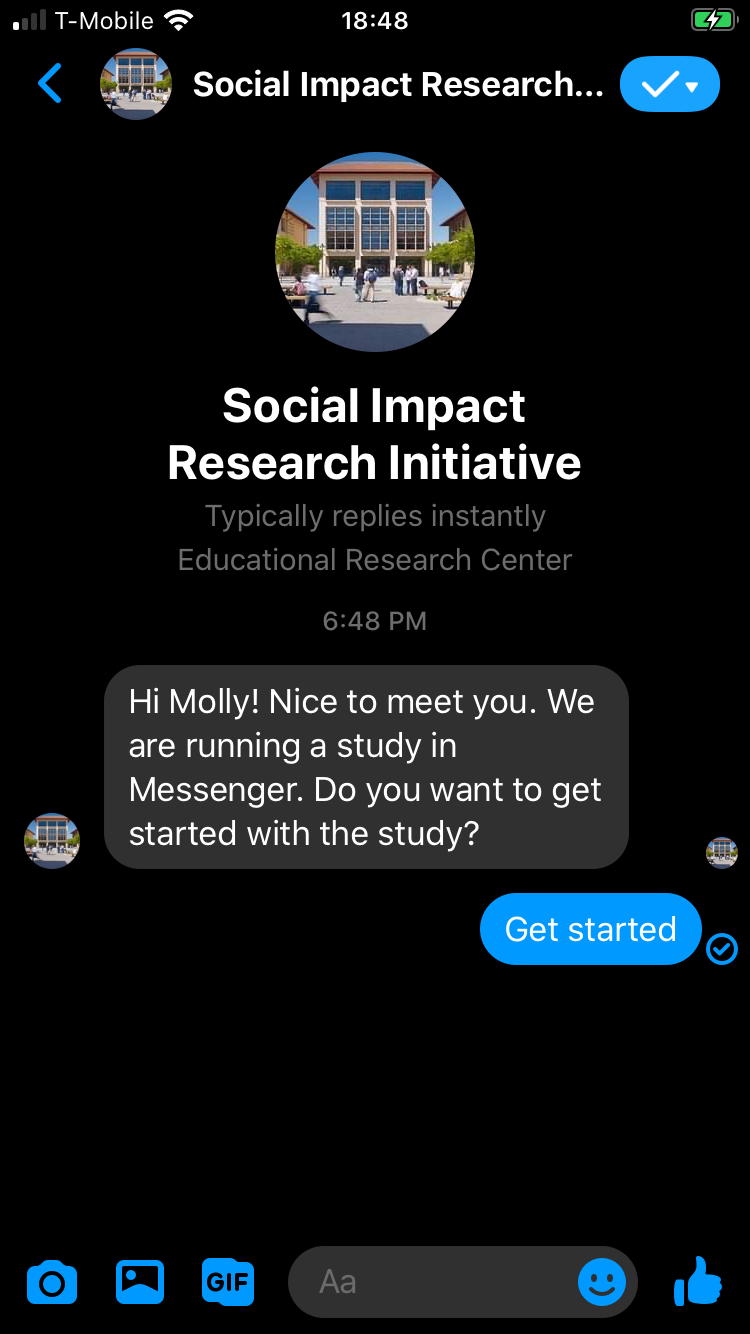
\includegraphics[width=.25\textwidth]{chatbot_image.png}
\end{figure}

\section{Survey and data}\label{appendix:data}
\subsection{Covariates}\label{appendix:covariates}
\todo{ADD new covariates to this table (belief, locus of control, etc.)}
\begin{table}[H]
\begin{adjustbox}{totalheight=.9\textheight-2\baselineskip, max width = \textwidth}
\begin{tabular}{p{0.3\linewidth}p{0.7\linewidth}p{0.25\linewidth}}
\textbf{Covariate}                   & \textbf{Response options} & \textbf{Coded as}                                     \\
\hline
Gender                                      & Male,   Female, Nonbinary, Other                           & 1 if male, 0 otherwise  \\
Age                                         & Integers                                                   & Continuous, {flag if greater than 120}              \\
Education &
  No   formal schooling, Informal schooling only, Some primary school, Primary   school completed, Some secondary school, Secondary school completed,   Post-secondary qualifications, Some university, University completed,   Post-graduate &
  1:10, flag if missing \\
Geography                                   & Urban, Rural                                 & 1 if urban, 0 otherwise \\
Religion                                    & Christian, Muslim, Other/None                           & Indicators              \\
Denomination (Christian)  & Pentecostal, Other  & Indicator (coded 1 if Pentecostal, 0 otherwise)\\
Religiosity   (freq. of attendance) &
  Never,   Less than once a month, One to three times per month, Once a week, More than   once a week but less than daily, Daily &
  1:6, flag if missing \\
%    Belief in God's control & 1. God will grant wealth and good health to all believers who have enough faith, 2. God doesn't always give wealth and good health even to believers who have deep faith & Indicator (coded 1 if answer is 1, 0 otherwise)\\
 Locus of control & 
% Some people feel they have completely free choice and control over their lives, while other people feel that what they do has no real effect on what happens to them. Please enter a number between 1 and 10, where 1 means "no choice at all" and 10 means "a great deal of choice" to indicate how much freedom of choice and control you feel you have over the way your life turns out 
[See survey instrument for full list] & 1:10, flag if missing\\
Index   of scientific views                 & [See   survey instrument for full questions and response options] & 0:2, flag if missing                     \\
Digital Literacy Index &  {[}Based on the first nine items of \cite{guessetal2020digital}'s  proposed measure, see  survey instrument for full questions and response options{]}& 0:24\\
Frequency of social media usage (x2)& {[}See   survey instrument for full questions and response options{]} & 0:3, flag if missing \\
Cognitive Reflection Test& {[}See   survey instrument for full questions and response options{]}& 0:3 (1 point for each correct response)\\
Index of household possessions%:   radio, tv, motorvehicle/motorcycle, computer/laptop, bank account, mobile   phone, bicycle 
&
  I/my household owns, Do not own [See survey instrument for items] &
  Continuous, sum of owned items, flag if all missing \\
Job   with cash income                      & Yes,   No                                                  & 1 if yes                \\
Number   of people in household             & Integers                                                   & Continuous, flag if missing              \\
Political affiliation & Governing party v. opposition & Indicator (coded 1 if associate with or voted for candidate from governing party, 0 otherwise)\\
Concern regarding COVID-19                  & Not at all worried, Somewhat worried,  Very   worried      & 1:3, flag if missing                     \\
%COVID-19 information & [Three True/False questions, see survey instrument for full questions] & 0:3 (1 point for each correct response)\\
Perceived government efficacy   on COVID-19 & Very   poorly, Somewhat poorly, Somewhat well, Very well   & 1:4, flag if missing \\
%Sources and frequency of news/media consumption &Never, Less than once a month, A few times a month, A few times a week, Once a day, Multiple times a day \ \  [See survey instrument for sources]  &  0:5 for \textit{each} of top three sources
{Strata of response to pre-test stimuli} & [Would share stimuli on timeline/via Messenger]& Indicators for strata (0:2) x (True + False = 2 types) $\times$ (timeline + Messenger = 2 channels) 
\end{tabular} 
\end{adjustbox}
\footnotesize
\textit{Note:} Regarding missingness flags, respondents must respond to chatbot questions to advance in the survey, but for contexts they may enter ``skip'' if they do not wish to answer a given question, with the exception of age, which we check is greater than 18. 
\caption{Covariates and response options}
\label{cov_long}
\end{table}

In all analyses, we include the pre-test response strata and indicators for individual stimuli.

\subsection{Survey Instrument}\label{appendix:survey}%\todo{Check for update to public-facing survey instrument.}
The survey script is available at this link:\\
\url{https://docs.google.com/spreadsheets/d/1ZEi8xU-TOZCZIQnDqq4VYjG5cWjIaWNyoKvPCjLL3fg/edit#gid=366167997&range=A1}

\subsection{Stimuli}\label{appendis:stimuli}
All of the stimuli used in the experiment are available at this link:\\
\url{https://docs.google.com/spreadsheets/d/1ZEi8xU-TOZCZIQnDqq4VYjG5cWjIaWNyoKvPCjLL3fg/edit?usp=sharing}


\subsection{Treatments}
%\todo{Include mockups for headlines, full questions for respondent-level treatments, add deliberation stimuli and describe}

\subsubsection{Facebook Tips}\label{sec:fbtips}
The script for the Facebook tips respondent-level treatment is as follows:

As we're learning more about the Coronavirus, new information can spread quickly, and it's hard to know what information and sources to trust. Facebook has some tips for how to be smart about what information to trust. 

1. Be skeptical of headlines. False news stories often have catchy headlines in all caps with exclamation points. If shocking claims in the headline sound unbelievable, they probably are.

2. Look closely at the link. A phony or look-alike link may be a warning sign of false news. Many false news sites mimic authentic news sources by making small changes to the link. You can go to the site to compare the link to established sources.

3. Investigate the source. Ensure that the story is written by a source that you trust with a reputation for accuracy. If the story comes from an unfamiliar organization, check their ``About'' section to learn more.

4. Watch for unusual formatting. Many false news sites have misspellings or awkward layouts. Read carefully if you see these signs.

5. Consider the photos. False news stories often contain manipulated images or videos. Sometimes the photo may be authentic, but taken out of context. You can search for the photo or image to verify where it came from.

6. Inspect the dates. False news stories may contain timelines that make no sense, or event dates that have been altered.

7. Check the evidence. Check the author's sources to confirm that they are accurate. Lack of evidence or reliance on unnamed experts may indicate a false news story.

8. Look at other reports. If no other news source is reporting the same story, it may indicate that the story is false. If the story is reported by multiple sources you trust, it's more likely to be true.

9. Is the story a joke? Sometimes false news stories can be hard to distinguish from humor or satire. Check whether the source is known for parody, and whether the story's details and tone suggest it may be just for fun.

10. Some stories are intentionally false. Think critically about the stories you read, and only share news that you know to be credible.



\subsubsection{AfricaCheck Tips}\label{sec:actips}
The script for the AfricaCheck tips respondent-level treatment is as follows:

As we're learning more about the Coronavirus, new information can spread quickly, and it's hard to know what information and sources to trust. AfricaCheck.org has some tips for how to be smart about what information to trust. 

1. Pause, particularly if the post, tweet or message makes you scared or angry. 

False or unverified information can spread quickly, especially if it makes you feel particular emotions.

2. Consider the source

When a friend or contact shares new information on Covid-19, it’s good to ask them: “How do you know that?” The answer can help you work out if they have first-hand knowledge of the information.

3. Try to find a trusted source

Check if fact-checking organisations have debunked the claim. For Covid-19, these are some good options:

First Draft\\
Africa Check\\
AFP Fact Check

\subsubsection{Accuracy and Deliberation Nudge Treatments}\label{sec:nudge}

For both the accuracy and deliberation nudge treatments, respondents will see the below placebo headline and asked the nudge question about it.For the accuracy nudge respondents are asked to think about whether the headline is true. The deliberation nudge asks respondents to think about why they would either choose to share or not share this headline.

\begin{figure}[htb]
\centering
    \begin{minipage}{0.45\textwidth}
        \centering
        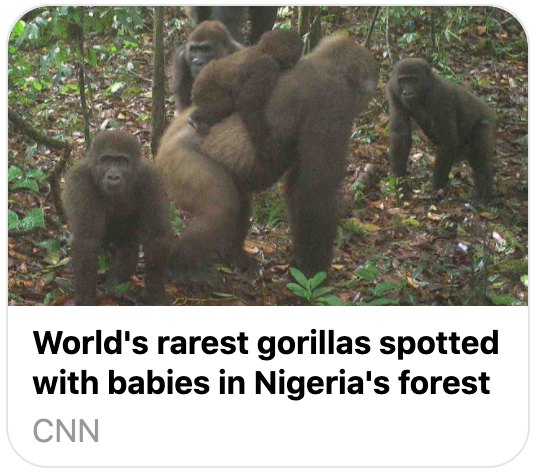
\includegraphics[width=\textwidth]{placebo_ng.png} 
        \caption{Placebo headline for Nigerian respondents}
    \end{minipage}\hfill
    \begin{minipage}{0.45\textwidth}
        \centering
        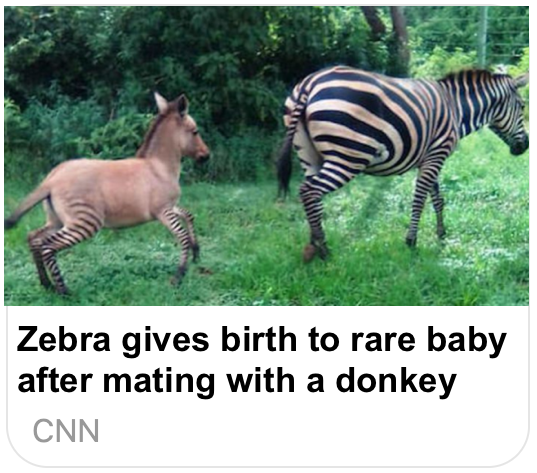
\includegraphics[width=\textwidth]{placebo_ky.png} 
        \caption{Placebo headline for Kenyan respondents}
    \end{minipage}
\end{figure} 

\FloatBarrier
\subsubsection{Pledge Treatment}
\label{sec:pledge}
This treatment draws on the psychological evidence around commitment and consistency \citep{cialdini1987influence,costa2018walking}. Knowing that people, as much as possible, want to appear consistent with their prior words and actions, we want to see whether we can first get them to commit to an ``easy ask'' and then lead them down a path towards a public (or private) pledge.


\begin{enumerate}

\item Do you want to keep your family, friends and community safe from COVID-19? (Yes!, No)
\\\textit{If "No" $\rightarrow$ end}

\item Did you know that false information about ways to prevent or cure COVID-19 threaten the health and well-being of everyone around us?  (Yes, No)

\item Are you committed to keeping your family, friends, and community safe from COVID-19 misinformation? (Yes!, No)
\\\textit{If "No" $\rightarrow$ end}

\item Great! Take our pledge by posting this image [here/to your timeline] now.
\\NOTE: \textit{Respondents are randomized to either be asked to take the pledge privately, within the chatbot, or to post the pledge publicly to their timeline.}

%\item IF 1=YES: Are you committed to stopping the spread of harmful/dangerous false information about COVID-19 online? (yes, no)
%\item IF 1=NO: Why not? [open response]
%
%\textit{Respondents in pledge treatment will be randomized (equal and static assignment probability) to either see the public or private pledge below}
%
%\item \textbf{public pledge:}\\
%IF 2=YES:  Great! Please take our pledge by posting this pledge to your timeline now. \\ IF 2=NO: Why not? [open response]
%
%\item \textbf{private pledge:}\\
%IF 2=YES:  Great! Please take our pledge now by posting it here. \\
%IF 2=NO: Why not? [open response]

\begin{figure}[htb]
\centering
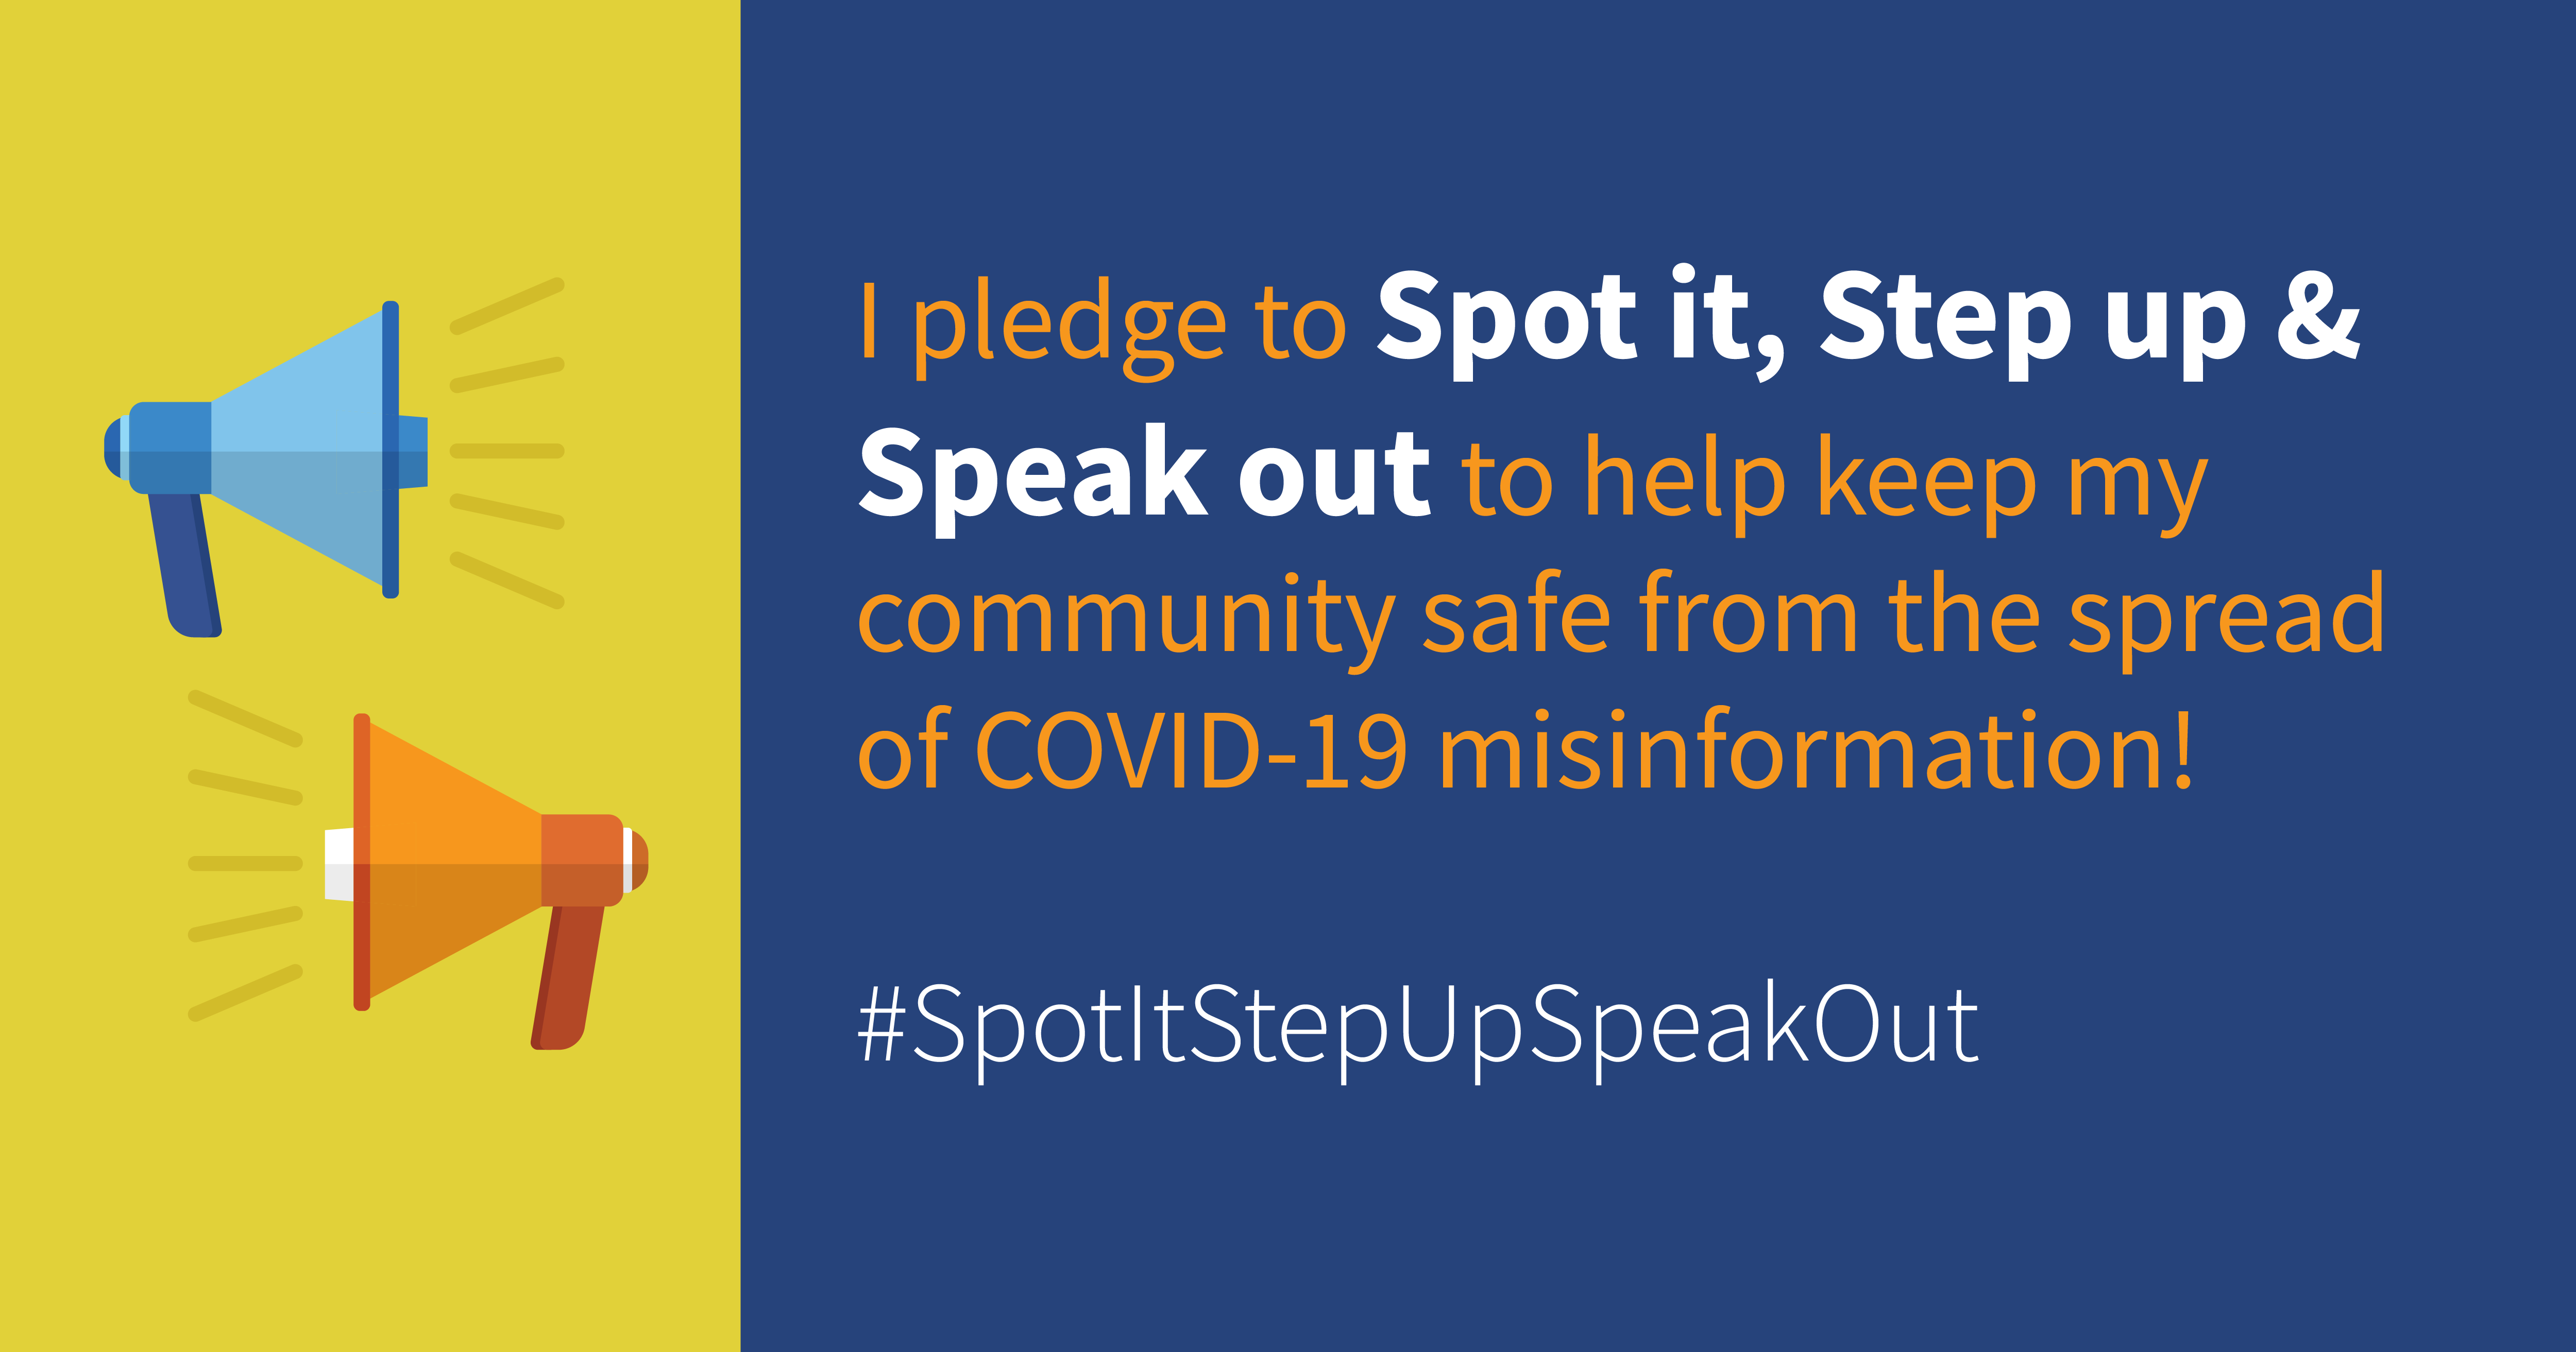
\includegraphics[width=.5\textwidth]{pledge_image.png}
\caption{Pledge infographic respondents are asked to post \textit{privately} to the chatbot or \textit{publicly} to their timeline.}
\end{figure}

\end{enumerate}

\subsubsection{Headline Level Treatments}
%Samples of the three headline-level treatments appear below:

\begin{figure}[htb]
\centering
    \caption{Headline treatments}
    \label{headline_treatments}
    \begin{minipage}{0.4\textwidth}
        \centering
        
\includegraphics[width=\textwidth]{treat_relatedarticles.png} 
        \caption*{Related Articles}
    \end{minipage}\hfill
    \begin{minipage}{0.4\textwidth}
        \centering
        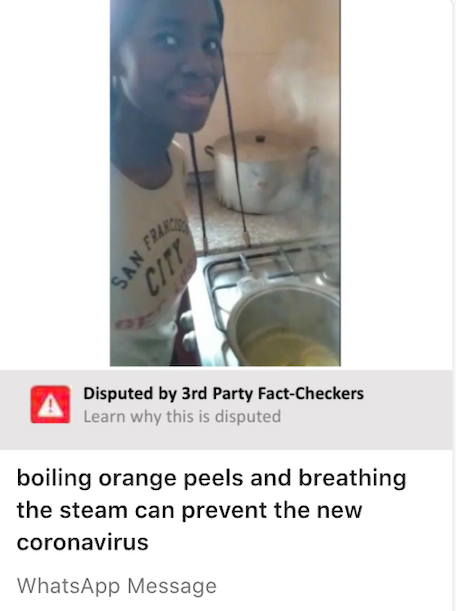
\includegraphics[width=\textwidth]{treat_factcheck.png} 
        \caption*{Factcheck}
    \end{minipage}
    \begin{minipage}{0.4\textwidth}
        \centering
        
\includegraphics[width=\textwidth]{treat_moreinfo.png} 
        \caption*{More information}
    \end{minipage}\hfill
     \begin{minipage}{0.45\textwidth}
        \centering
        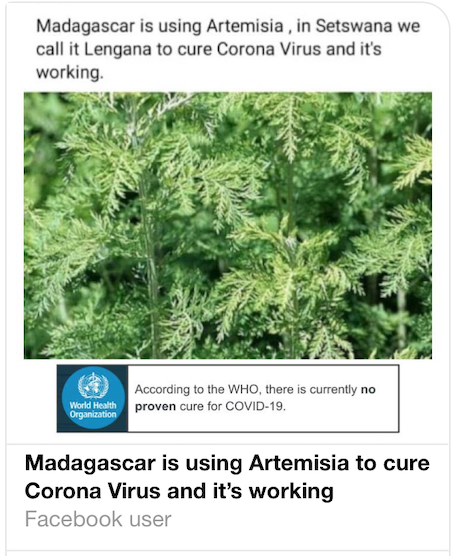
\includegraphics[width=\textwidth]{treat_realinfo.png} 
        \caption*{Real information}
    \end{minipage}
\end{figure}

\FloatBarrier
\section{Batch-wise balanced linear Thompson sampling}\label{appendix:agent}

A note on notation: while $X_i$ represents the covariates observed for individual $i$, the covariate vector $X_{[W]i}$ is in the appropriate format for the relevant counterfactual treatment indicators and interactions.


\begin{algorithm} \footnotesize
    \caption{Batch-wise balanced linear Thompson sampling}
    \label{algg:bblts}
    \begin{algorithmic}[1] % The number tells where the line numbering should start
    	\State$\Xi_w \leftarrow$ empty matrix; $\X_w \leftarrow$ empty matrix; $r_w \leftarrow$ empty vector for $w \in \ww$. 
	\Comment{Initialize weight matrices, covariate matrices, and reward vectors, for each treatment condition separately. Denote the control condition $w_{C}$. }
    	\For{$i = 1, \dots, N$}
		\If{$i \in \mathcal{I}_1$}
			 \State $e_{w}(X_i) \leftarrow \frac{1 }{|\ww| } \ \ \forall w \in \ww $ 
		\ElsIf{$i \in \mathcal{I}_b$ for $b = 2, \dots, B-1$}
			\If{$i$ is the first observation in $\mathcal{I}_b$}
				\For{$w\in \ww$}
					\State $B_w \leftarrow X^\top \Xi_w X + \lambda^{CV} \mathbf{I}$ 
					\State $\hat\theta_{w} \leftarrow B_w^{-1} X_w^\top \Xi_w r_w$
					\State $\hat\V[\hat\theta_{w}] \leftarrow B_w^{-1} \left(\left( r_w - X_w^\top\hat\theta_{w} \right)^\top \Xi_w \left( r_w - X_w^\top\hat\theta_{w} \right)\right)$
				\EndFor
			\EndIf
			\For{$m = 1, \dots, M$}
				\State Sample $\tilde \theta ^{(m)}_w \sim \mathcal{N}\left(\hat\theta_{w}, \hat\V[\hat\theta_{w}] \right) \ \   \forall w \in \ww$
			 \EndFor
				\State $q_w(X_i) \leftarrow \frac{1}{M} \sum_{m=1}^M 1\left\{ w = \underset{w}{\argmax} \{ X_{[1]i}^\top \tilde \theta ^{(m)}_1, \dots, X_{[|\ww|]i}^\top\tilde \theta_{|\ww|}^{(s)} \}  \right\}$ \Comment{ Compute TS probabilities.}
			\State $\tilde{q}_{w_C}  \leftarrow 1/|\ww| + {q}_{w_C}/(1-1/|\ww|) $ \Comment{Augment the control with a fixed probability. }
                         \State $ \tilde{q}_w(X_i)  \leftarrow\max\Biggr\{\frac{ q_{i}(w)}{(1-1/|\ww|)} , p\Biggr\} \ \ \forall w \in \ww \setminus \{w_C\}$ \Comment{Impose floors on remaining probabilities. }
                          \State $e_{w}(X_i) \leftarrow \frac{ \tilde{q}_w(X_i)}{\sum\limits_{w \in \ww }\tilde{q}_w(X_i) } \ \ \forall w \in \ww $ \Comment{Ensure probabilities sum to 1.}  
		\EndIf
		\State Assign $w_i \sim \textrm{Multinom}( e_{1}(X_i) , \dots,  e_{|\ww|}(X_i) )$
		\State $\xi^{IPW}_w(X_i) \leftarrow \frac{ 1 }{e_{w}(X_i)}$ \Comment{Assign inverse probability weights.}
		\State $\Xi_{w_i} \leftarrow \diag \left(\Xi_{w_i}, \xi_i\right)$ \Comment{Augment relevant weight matrix.}
		\State $\X_{w_i} \leftarrow [\X_{w_i}:x_{w_i}^\top]$ \Comment{Augment relevant covariate matrix.}
		\State $r_{w_i} \leftarrow  [r_{w_i}: y_i]$ \Comment{Augment relevant reward vector.}

	\EndFor
    \end{algorithmic}
\end{algorithm}

\clearpage


\section{Estimation Considerations}

\subsection{Inverse probability weighting} \label{appendix:stabilized}
Inverse probability weighted estimation typically uses weights as follows, 
\begin{align*}
\xi^{IPW}_w(X_i) = \frac{ 1 }{e_{w}(X_i)} \label{eq:IPW} \numberthis\\
e_{w}(x) = \Pr[W_i = w|X_i = x].
\end{align*}
Here, we could directly plug in the respective treatment assignment probabilities from the experimental design for the $e_{w}(X_i)$. 

In ex post evaluation, we use the stabilized version of these weights, normalizing weights to sum to one on the empirical data. This may improve RMSE of the estimator \citep{cole2008constructing}. 
\begin{align}
\left.
\xi^{SIPW}_w(X_i) = \frac{ 1 }{e_{w}(X_i)}
\middle/ 
{ \sum_{j = 1}^N \frac{1\{W_{j} = w\}}{e_{w}(X_j)} } \label{eq:SIPW} \numberthis
\right.
\end{align}

For adaptively collected data we use cumulative moving stabilized weights. If data were collected in an online manner (i.e., if Thompson sampling probabilities were updated with each observation), $N$ in the above formula would be replaced by $i$. In the batched version, all observations in the same batch share the same history, and so instead, we sum over all observations in batches \textit{up to and including} the batch that includes observation $i$. \todo{Could formalize this.}

\begin{align}
\left.
\xi^{SIPW}_{b,w}(X_i) = \frac{ 1 }{e_{w}^{\pi^{(b)}}(x)}   
\middle/ 
{ \sum_{j = 1}^T \frac{1\{W_{j} = w\}}{e_{w}^{\pi^{(B_j)}}(X_i)} } \label{eq:IPW} \numberthis
\right.
\end{align}

\subsection{Random forest estimation}\label{appendix:grf}
For policy learning and evaluation, we estimate conditional means using generalized random forests, as implemented by the \texttt{grf} package in \texttt{R} \citep{Tibshirani:2020aa}. 

For a given dataset, we estimate conditional means under each treatment condition $w$:
\begin{enumerate}
\item Fit a random forest estimator on the observations assigned $w$ . 
\item For observations assigned $w$, calculate $\hat\mu_w(X_i, W_i = w)$ using out-of-bag predictions. 
\item For observation not assigned $w$, calculate $\hat\mu_w(X_i, W_i \neq w)$ using regression forest predictions from the model in step 1. 
\end{enumerate}

\subsection{Adaptively weighted doubly-robust estimation} \todo{Add appropriate reference to LFO paper.}\label{appendix:DRlfo}
For adaptively collected data, we use doubly robust scores as in (\ref{eq:DR}), but due to the dependent nature of the data, to avoid bias, we must ensure that we use only historical data in our estimates. This means that in each batch we estimate the nuisance components only using data up to and including the current batch. 

To estimate conditional means, we follow the steps above in \ref{appendix:grf}, with minor adjustments. For each batch $b$ in $b = 1, \dots, B-1$ and for each treatment $w$:
\begin{enumerate}
\item Fit a random forest estimator on the observations assigned $w$ in batches up to and including batch $b$. 
\item For observations assigned $w$ in batch $b$, calculate $\hat\mu_w(X_i)$ using out-of-bag predictions. 
\item For observation not assigned $w$ in batch $b$, calculate $\hat\mu_w(X_i)$ using regression forest predictions from the model in step 1. 
\end{enumerate}

We use the cumulative moving version of the stabilized inverse probability weights from (\ref{eq:SIPW}), substituting the current maximum index value for $N$. 
Doubly robust scores are then formed from the relevant component parts. 


\subsection{Random best fixed policies}\label{appendix:bestfixed}
We are interested in learning and evaluating the best fixed policy. However, if we learn which fixed policy is best by taking the fixed policy with the highest mean, we get a biased estimate of the best fixed policy. To see this, consider:
\begin{align*}
\E[\max(X_1, \dots, X_N)] \ge \max(\E[X_1],\dots, \E[X_N]). 
\end{align*}

To address this concern, we consider instead a \textit{random} best fixed policy. 
\begin{enumerate}
\item For each observation $i>1$ in the experiment, we calculate the value of fixed policies as the average of scores up to time $i-1$. 
\begin{align*}
\hat{V}_{i-1}({\pi}_{w})  &:= \frac{1}{i-1 } \sum_{j = 1 }^{i-1} \hat{\Gamma}_{j,w} \quad \text{for fixed policies $w$}
\end{align*}
\item The ``best'' fixed policy in period $i$ is the treatment with the highest estimate:
\begin{align*}
w_i^* =  \argmax_w \ \hat{V}_{i-1}({\pi}_{w})
\end{align*}
\item The score for the random best fixed policy in time $i$ is then the score in that period for the selected arm, $\hat{\Gamma}_{i, w^*}$ 
 \item To evaluate the policies, we again take the average scores. The evaluation set $\mathcal{I}^*$ will be the entire data set for data collected under the procedures for the random agent as described above in Section~\ref{randomlearning}, and up through batch $B-1$ for data collected under the procedures for the adaptive agent--excluding the first observation. 
    \begin{align*}
          \hat{V}(\hat{\pi}_{w^*})  &:= \frac{1}{\big{\lvert} \mathcal{I}^* \big{\rvert}} \sum_{i \in \mathcal{I}^* } 
          \hat{\Gamma}_{i, w_i^*} 
  \end{align*}
\end{enumerate}




\end{document}